\documentclass{article}

\usepackage{iclr2026_conference,times}
\usepackage{amsmath,amssymb,booktabs,graphicx,microtype,array,tabularx}
\usepackage{float}
\usepackage[hidelinks]{hyperref}
\usepackage{url}

% Float placement: a float must fill 90% of a page before it may claim a float
% page of its own, and any float page starts flush at the top instead of being
% vertically centred.  This keeps large tables on text pages and removes the
% empty bands that vertically centred float pages leave above and below.
\renewcommand{\floatpagefraction}{0.90}
\renewcommand{\bottomfraction}{0.50}
\makeatletter
\setlength{\@fptop}{0pt}
\setlength{\@fpbot}{0pt plus 1fil}
\makeatother

% Anonymous initial submission: do not enable \iclrfinalcopy.
% \iclrfinalcopy
\newcommand{\Pfmt}{P(\mathrm{fmt})}
\newcommand{\PcFmt}{P(\mathrm{correct}\mid\mathrm{fmt})}
\newcommand{\pp}{\,\mathrm{pp}}
\newcommand{\good}{\textsc{survives}}
\newcommand{\blocked}{\textsc{not comparable}}

\title{Leveling Judge Stringency: What Survives a\\
Two-Bed Fallback-Rescue Format Artifact?}
\author{Anonymous authors}

\begin{document}
\raggedbottom
\maketitle

\begin{abstract}
Answer parsers are part of an evaluation's measurement instrument: a permissive
fallback can rescue a correct value without the requested explicit format.  We
audit this effect on two frozen beds by separating format coverage, accuracy
conditional on explicit format, and their strict joint product.  Both beds use
the free-form generative GSM8K split (no multiple-choice wrapper
is defined in the frozen artifacts; option-count and chance-rate baselines are
therefore not applicable), so cross-bed levels are selected-population
descriptions rather than capability rankings.  On every Bed~1 arm, the format
channel is $5.8$--$9.5\pp$ higher, far too small to explain the
$35$--$67\times$ rescue-ratio contrast.  Order is rule-dependent: the raw
point-estimate rule gives $3/28$, whereas the favorable paired
gate---pre-registered in estimand wording but operationalized post hoc---gives
$0/23$ and is scoped only to these two beds.  These $F_{\mathrm{strip}}$
counts use, respectively, the raw identifiable-pair and paired-definite
calibers; the separately reported adversarial planned-arm bounds use distinct
gated and raw-plan denominators (Table~\ref{tab:j2-gates}), and the
denominators are not interchangeable.  The registered pattern question is
\textsc{not\_identified} from the shipped summaries: the data cannot decide,
and the primary conditional MDA80 is not identified.\footnote{The reported
conditional CI half-width gives a retrospective, post-hoc normal-approximation
resolution of $\approx4.57\pp$; it is not a shipped or preregistered MDA80 and
is distinct from the canonical/strict secondary rulers.  A same-bed
regex-parser lineage sensitivity appears in Appendix~\ref{sec:appx_parser}.}
\end{abstract}

\section{Introduction}
\label{sec:intro}

Evaluation code is part of the measurement instrument.  When a parser first
looks for an explicit answer format and then rescues an otherwise unparseable
response from its final position, the reported accuracy mixes at least two
events: producing the requested format and answering correctly within that
format.  A comparison is especially fragile when different experimental beds
invoke the rescue path at very different rates.

We study this failure mode in two frozen beds evaluated by canonical v1.1.
Table~\ref{tab:rescue} makes the central contrast reconstructible: the rescue
share differs by $35$--$67\times$ between \textsc{B1-32} and the three Bed~2
arms used in the primary level/pattern analyses.  This prevents a raw
canonical level from carrying the same operational meaning across beds, but
does not imply that every relation measured by the judge disappears.
\begin{table*}[!h]
\centering\footnotesize
\setlength{\tabcolsep}{3pt}
\begin{tabular}{@{}lcccccccl@{}}
\toprule
arm & bed & canonical & strict & formatted & rescue & rescue share & Wilson $95\%$ CI & role \\
\midrule
\textsc{B1-32}  & 1 & $604/1319$ & $69/1319$  & $131/1319$ & $535$ & $88.58\%$ & $[85.79,90.87]$ & headline/J1 \\
\textsc{B2-96}  & 2 & $303/356$  & $299/356$ & $350/356$  & $4$   & $1.32\%$  & $[0.51,3.34]$   & J1 primary \\
\textsc{B2-128} & 2 & $636/712$  & $623/712$ & $698/712$  & $13$  & $2.04\%$  & $[1.20,3.47]$   & J3 baseline \\
\textsc{B2-160} & 2 & $318/356$  & $310/356$ & $347/356$  & $8$   & $2.52\%$  & $[1.28,4.88]$   & J3 contrast \\
\bottomrule
\end{tabular}
\caption{Headline fallback-rescue contrast on free-form, generative GSM8K
items (there is no multiple-choice option set or chance-rate baseline).  The
explicit \emph{bed} column is the first occurrence of each arm name and fixes
the cross-bed reading: \textsc{B2-96}/\textsc{B2-128}/\textsc{B2-160} are Bed~2
dose arms, whereas the numeral after B elsewhere indexes a configuration-cell
family rather than a bed (Table~\ref{tab:vocabulary}).
Canonical is fallback-inclusive;
strict removes fallback; rescue share is $\mathrm{rescue}/\mathrm{canonical}$.
The Bed~1 row compared with the three primary Bed~2 rows yields
$88.58/2.52=35.2\times$ to $88.58/1.32=67.1\times$.  Wilson endpoints use
one half-up rounding rule; the two additional
Bed~2 dose arms are included in the complete J2 inventory
(Table~\ref{tab:bed2-j2}), not silently generalized into this three-arm range.}
\label{tab:rescue}
\end{table*}

This paper separates three questions that are often conflated:
\begin{enumerate}
  \item \emph{Level:} can normalized accuracies be read as a cross-bed
        capability ordering?
  \item \emph{Order:} does removing fallback ever reverse an observed strict
        ordering between arms?
  \item \emph{Pattern:} does a registered canonical-tie/strict-separation
        label revert to a tie after judge normalization?
\end{enumerate}
Our contribution is a measurement audit with \emph{pre-registered estimands
and primary-arm assignment}; the favorable order gate and final synthesis were
pre-registered in their estimand wording but operationalized post hoc, with
every deviation logged in Appendix~\ref{sec:appx_deviations}.  The result is
deliberately asymmetric: level remains inadmissible as a capability ordering;
order must be read under both the raw-sign and favorable paired-gate rules; and
the registered tie pattern is \textsc{not\_identified} from the shipped
summaries on its primary estimand---the data cannot decide, which is not a
proof of no effect.

\section{Beds, arms, and rulers}
\label{sec:beds}

An evaluation \emph{bed} is a frozen generator, dataset, decoding
configuration, and judge.  Our two beds share one generator:
LLaDA-8B-Instruct, a discrete
masked diffusion language model \citep{nie2025llada}
(official checkpoints \texttt{GSAI-ML/LLaDA-8B-Instruct}).  The generation
records are frozen artifacts from the cited trials; decoding budgets are
listed per arm below, and sampling seeds and temperatures are not recorded
in the frozen artifacts, so we disclose that as a provenance gap rather than
retrofit values our records cannot certify
(\S\ref{sec:repro}).  Two-bed independence
here is split-disjointness plus a different manipulated axis, not a
cross-model claim; a cross-generator law is out of scope.

\textbf{Bed 1.}  The LLaDA generator evaluated the 1{,}319-item generative
GSM8K test split \citep{cobbe2021gsm8k}.  Although earlier project records
used the alias ``GSM8K-MC,'' the frozen source contains the original free-form
questions and no option set; no multiple-choice wrapper, option count, or
$1/K$ chance baseline is therefore defined.  We retract the earlier
``above-chance'' wording and assess the two extraction channels only against
each other.
Its arms differ in their generation token budget: the matched arms
\textsc{B1-32}/\textsc{B1-64}/\textsc{B1-128}/\textsc{B1-256} use
exactly 32, 64, 128, and 256 generation tokens (cells
\texttt{b1\_matched\_*}), and \textsc{B0-256} is a fixed-256 control
(\texttt{b0\_fixed\_256}).  Three holdout arms probe budgeted
alternatives: \textsc{H-PRED-95} decodes to a prediction-side final length of
95 tokens; \textsc{H-DAEDAL-1024}\footnote{Historical project records call
this arm \textsc{B2-DAEDAL} (Bed~1); the \textsc{H-} prefix prevents collision with
Bed~2 dose-arm names.} decodes with the DAEDAL
\citep{li2025daedal} training-free dynamic length-expansion rule under a
1024-token ceiling; and \textsc{H-VAR} stops at a variable per-item budget.
Artifact-key mappings are confined to the
Appendix~\ref{sec:appx_artifact} provenance ledger.

\textbf{Bed 2 (train-short-B).}  The same LLaDA generator on the GSM8K
training split short-band ($n=712$ items; length coefficient of variation
$0.049$), evaluated autoregressively.  Its arms are dose arms spanning
\emph{five} token budgets---64, 96, 128, 160, and 192---from two paired audit
trials: one supplies the 96/160 arms and reuses the fixed-128 run, while the
other supplies the 64/192 arms (each half-arm has $n{=}356$).  Exact trial and
artifact identifiers are confined to Appendix~\ref{sec:appx_artifact}.
The level and pattern analyses center on \textsc{B2-96}/\textsc{B2-128}/
\textsc{B2-160}; all five dose arms enter the J2 inventory.  A
whitelist-robustness property
matters for the fallback channel on
this bed: every unformatted Bed~2 row is also strict-wrong, so stripping the
fallback changes nothing on the auxiliary strict numerator; the
constructional part of this invariance is described in \S\ref{sec:limitations},
and its data-dependent remainder must be retested on a new bed.

\textbf{Rulers.}  The canonical judge v1.1 checks candidates in priority
order: the scaffold \texttt{\#\#\#}, then \texttt{\textbackslash boxed\{\}}, then a
final-position fallback that rescues the last numeric span.  The strict ruler
accepts only the first two (the \texttt{hash}/\texttt{boxed} whitelist).  A
\emph{rescue} is an output judged correct by the canonical ruler only via the
final-position fallback.  Single-proportion intervals throughout this paper are
Wilson intervals; two-proportion differences use normal intervals.

\begin{table*}[!tb]
\centering\footnotesize
\setlength{\tabcolsep}{2pt}
\begin{tabular}{@{}cl>{\raggedright\arraybackslash}p{4.95cm}%
                    cl>{\raggedright\arraybackslash}p{4.95cm}@{}}
\toprule
symbol & & definition & symbol & & definition \\
\midrule
$F,C$ && explicit-format and strict-correct events & $q,a,s$ && $P(F)$, $P(C\mid F)$, and $P(C\cap F)=qa$ \\
$m,B$ && discordant-pair count and bootstrap replicates & $u$ && unformatted B2-128 items on J3 common support \\
$F_{\mathrm{strip}}$ && definite canonical relations whose strict sign reverses & MDA80 && minimum detectable absolute effect at 80\% power \\
$\Delta_{\mathrm{can}},\Delta_{\mathrm{strict}}$ && arm-A minus arm-B gaps under canonical/strict rulers & $\Delta_{\mathrm{true}}$ && J3 primary conditional gap, $a_{160}-a_{128}$ \\
$b$ && $P(\mathrm{canonical\ correct}\mid\neg F)$, the fallback channel & S1, S2 && tight-correct / raw-whitelist strict-cell sources \\
\bottomrule
\end{tabular}
\caption{Compact vocabulary used throughout.  All $\Delta$ values are raw
percentage points; ``true'' distinguishes the primary conditional estimand
from the fallback-inclusive canonical ruler, not a causal effect.  The numeral
after B indexes a configuration-cell family, not a bed: Bed~2 dose arms use
\textsc{B2-$\langle$size$\rangle$}, whereas the historical
\textsc{B2-DAEDAL} name denotes a Bed~1 holdout (renamed
\textsc{H-DAEDAL-1024} here).}
\label{tab:vocabulary}
\end{table*}

\subsection{Related work and closest-work map}
\label{sec:related}

The beds use GSM8K-derived items \citep{cobbe2021gsm8k} and LLaDA
\citep{nie2025llada}; dLLM generation and acceleration methods change decoding
or compute rather than the downstream answer parser
\citep{zhou2026dllm,ye2025dream,li2025daedal,wu2026dreamon,wu2025fastdllm,wu2025fastdllmv2}.
Zheng et al. \citep{zheng2023judging} belongs to the separate LLM-as-judge
thread and is not evidence for deterministic extraction.

The closest extraction work is Jo et al. \citep{jo2025finding}, who sweep
judges and prompts over reasoning traces and show that where an answer is found
can change reported performance.  xFinder \citep{yu2024xfinder} directly
targets key-answer extraction and reports failures of regex-based evaluation
harnesses.  Our narrower delta is empirical: we isolate a frozen
parser-fallback rescue path, decompose its reported score, and compare the
xFinder regex tier on the same two beds; we do not test xFinder's learned tier
or Answer Regeneration.  In selective prediction, coverage and conditional
accuracy are standard paired quantities in the risk--coverage trade-off
\citep{elyaniv2010selective}.  Equation~\ref{eq:factorization} is therefore a
probability identity, not a novelty claim; the contribution is its registered
co-report and its use to audit this specific parser artifact.
Table~\ref{tab:closest-work} is the positioning boundary: it anchors each
component to verified Jo/xFinder/selective-prediction precedents and does not
turn the regex-tier reparse into a same-bed comparison with xFinder's learned
tier or Answer Regeneration.

The inferential pieces are likewise standard.
\emph{(i) Format-emission base rate.}  The format share $q=P(\mathrm{fmt})$
and Wilson score intervals~\citep{wilson1927probable} summarize how often the
judge must fall back; exact binomial limits are from Clopper and
Pearson~\citep{clopper1934use}.
\emph{(ii) Correctness given format.}  Conditional contrasts
$a=P(\mathrm{correct}\mid\mathrm{fmt})$ are judged per-pair with McNemar's
paired test~\citep{mcnemar1947note}, with item-paired bootstrap intervals; we
explicitly decline a post-hoc equivalence claim, so the post-hoc $0.5$~pp tolerance is
reported without a formal
TOST~\citep{schuirmann1987comparison}, and family-wise control across the
tested definite pairs uses Dunn's multiple-comparison
correction~\citep{dunn1961multiple}.  Conditioning on format emission---a
post-generation property of the scored string---opens a collider-type,
selected-population contrast~\citep{elwert2014endogenous}, which is why J1 is
scoped as descriptive rather than a capability claim.
\emph{(iii) Evaluation hygiene.}  Answer-extraction rules measurably move
reported math-reasoning scores~\citep{jo2025finding,yu2024xfinder}, and our
preregister-then-report workflow follows calls for ML
preregistration~\citep{forde2019scientific}.  Within this neighborhood our
narrower contribution is the auditable factorization $s=q\,a$ and the
reported rule-pair for one fallback parser; we make no priority claim.

\begin{table*}[!t]
\centering\footnotesize
\setlength{\tabcolsep}{3pt}
\begin{tabular}{@{}>{\raggedright\arraybackslash}p{2.6cm}
                    >{\raggedright\arraybackslash}p{2.6cm}
                    >{\raggedright\arraybackslash}p{3.5cm}
                    >{\raggedright\arraybackslash}p{2.1cm}
                    >{\raggedright\arraybackslash}p{2.2cm}@{}}
\toprule
Component & Closest prior work & Difference here & Class & Evidence \\
\midrule
Extraction changes reported scores & Jo et al.; xFinder \citep{jo2025finding,yu2024xfinder} & Frozen fallback-rescue path plus same-bed regex-lineage audit & standard phenomenon; artifact-specific audit & Tables~\ref{tab:rescue}, \ref{tab:parser-lineage} \\
$q$, $a$, and $s{=}qa$ & Selective prediction \citep{elyaniv2010selective} & Registered co-report before any capability reading; identity itself is standard & standard identity; executed audit & Table~\ref{tab:j1-decomposition} \\
Paired order audit & McNemar and multiplicity control \citep{mcnemar1947note,dunn1961multiple} & Raw-first rule-pair; gate pre-registered in estimand wording, operationalized post hoc & standard tests; reporting protocol & Table~\ref{tab:j2-gates} \\
Deviation ledger & Forde \& Paganini \citep{forde2019scientific} & End-to-end executed instance with falsification criteria & standard practice; artifact audit & App.~\ref{sec:appx_deviations} \\
Selected-population level block & Collider literature \citep{elwert2014endogenous} & Measured two-bed rescue-share gap and its consequence & standard theory; artifact audit & Table~\ref{tab:rescue} \\
\bottomrule
\end{tabular}
\caption{Closest-work comparison at component level.  ``Standard'' denotes a
component already present in cited work; ``artifact audit'' denotes a property
of these frozen beds.  No priority is claimed beyond this verified neighborhood.}
\label{tab:closest-work}
\end{table*}

\paragraph{Claim-to-closest-work map.}
The level claim instantiates standard selection reasoning
\citep{elwert2014endogenous}; only its measured magnitude is artifact-specific.
The order tests are standard \citep{mcnemar1947note,dunn1961multiple}; the
raw-first rule-pair is our reporting choice.  The pattern claim instantiates
the extraction-sensitivity phenomenon \citep{jo2025finding,yu2024xfinder}; its
\textsc{not\_identified} verdict is specific to
Table~\ref{tab:j3-estimands}.  Finally,
the audit discipline follows \citet{forde2019scientific}, while the executed
deviation ledger is an artifact of this study.

Figure~\ref{fig:teaser} summarizes the measurement flow and keeps the three
audit conclusions visually separate; it is conceptual rather than numerical.

\begin{figure*}[t]
  \centering
  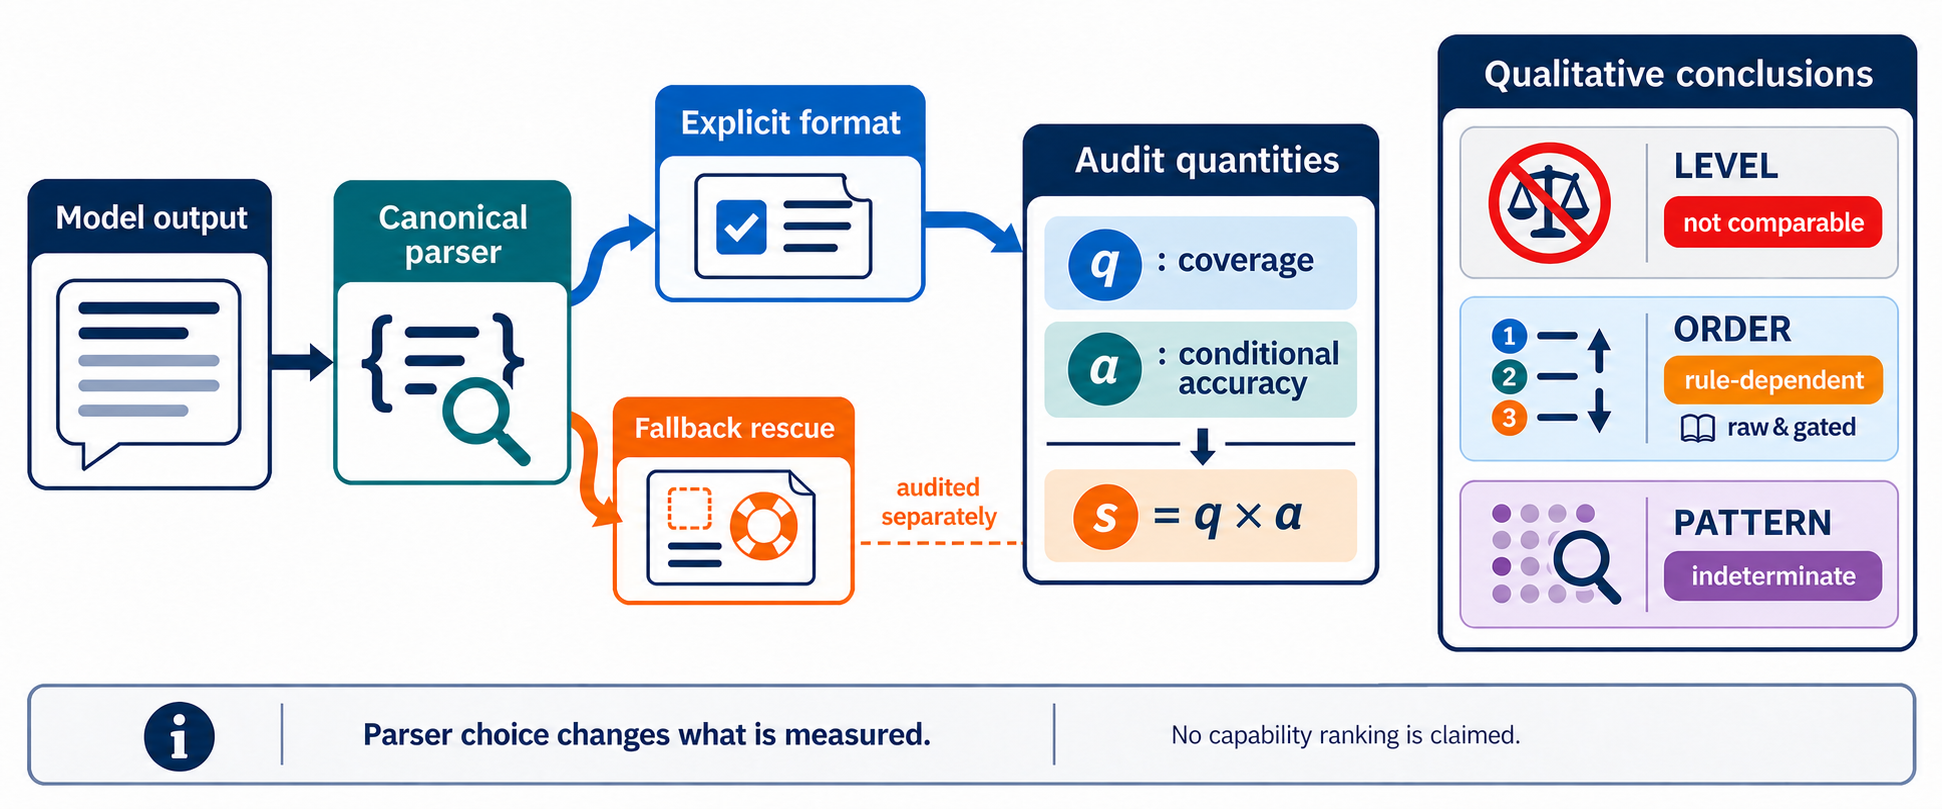
\includegraphics[width=\textwidth]{figures/judge_normalization_teaser.png}
  \caption{\textbf{Conceptual overview; not quantitative evidence.}
  Both beds enter the same canonical judge. The format audit exposes explicit-format
  and fallback-rescue channels before separating the three audit conclusions:
  level is not comparable; order leads with the raw rule and co-reports a
  favorable paired gate pre-registered in estimand wording but operationalized
  post hoc; and pattern is \textsc{not\_identified} on the registered primary
  estimand.  The badge reading ``indeterminate'' denotes exactly that verdict:
  the data cannot decide from the shipped summaries, which is not a proof of no
  effect. No counts are encoded; all measurements appear in
  Figure~\ref{fig:summary} and Table~\ref{tab:judgments}.}
  \label{fig:teaser}
\end{figure*}

\section{Judge normalization}
\label{sec:method}

\subsection{Events, estimands, and the exact identity}

The observational unit is an item-level binary record.  Let $F$ denote that
the answer uses an accepted explicit format, here the whitelist
\texttt{judge\_format}$\in\{\texttt{hash},\texttt{boxed}\}$, and let $C$ denote
a correct strict judgment.  We report two estimands:
\begin{align}
  a &\equiv \PcFmt, &&\text{primary, conditional on the scored format channel},
  \label{eq:conditional}\\
  s &\equiv P(C\cap F), &&\text{auxiliary, fallback-stripped over all items}.
  \label{eq:strict}
\end{align}
Writing $q\equiv\Pfmt$ gives the exact factorization
\begin{equation}
  s=q\,a.
  \label{eq:factorization}
\end{equation}
For reconstruction of the fallback-inclusive ruler, define
$b\equiv P(\mathrm{canonical\ correct}\mid\neg F)$; then canonical accuracy is
$qa+(1-q)b$.  This descriptive identity does not make $b$ part of the strict
joint estimand $s$.
The two estimands are complementary, not replicas.  The conditional $a$
describes correctness within the formatted subset, whereas $s$ charges a
system for failing to emit the format.  $s$ also charges a system for every
answer the fallback rescued: on \textsc{B1-32} it counts all $535$
fallback-corrected answers as wrong.  Across Bed~1 the fallback channel is only
$5.8$--$9.5\pp$ below the format channel (\S\ref{sec:channels}); on a
fallback-dominated arm, reporting both factors of $s=qa$ is therefore needed
to expose whether a canonical level is driven by answer correctness, format
emission, or rescue.

\subsection{Why conditioning does not create a common scale}
\label{sec:selection}

Conditioning removes the fallback channel but changes the population.  Format
emission is a \emph{post-outcome (post-generation) behavior}: the judge decides
$F$ and $C$ from the same generated string.  Selecting on $F$ can therefore
induce a selected-population (collider-type) contrast when response properties
associated with correctness also affect explicit formatting; it is not clean
pre-treatment stratification.  Across
Bed~1 arms, $q\in[0.0993,0.2661]$; on Bed~2,
$q\in[0.9747,0.9831]$. Thus Bed~1's conditional accuracy describes a formatted
subset comprising roughly $10$--$27\%$ of its items, while Bed~2's describes
nearly all items.
Unless formatting is ignorable or common support is restored, comparing the
two $a$ values is a selected-population contrast.  It is useful as a
sensitivity diagnostic but not as a pure capability scale.  The beds also
differ in prompt and task, adding an inseparable task confound.  Accordingly,
all contrasts below are decoding-budget~$\times$~task-format comparisons on a
single fixed model, not comparisons of model capability.

\subsection{Predicate correction and provenance}

An earlier implementation used the truth value of
\texttt{judge\_format}.  Because the sentinel string \texttt{none} is
nonempty, this predicate failed open and made $q=1$.  The frozen analysis uses
whitelist membership instead.  The formatted and strict columns of
Table~\ref{tab:rescue} give its independent recovery for all three Bed~2 arms.
The auxiliary
numerator is unchanged here because every unformatted row is also strict-wrong;
that property is at least partly constructional (the strict numerator is a
whitelist-conditioned count, \S\ref{sec:limitations}), and the data-dependent
remainder is not a general property of fallback stripping.

\section{Analysis plan and disclosed revisions}
\label{sec:analysis}

Table~\ref{tab:supports} inventories the frozen supports used by the primary
comparisons.  Critically, Bed~2's contrast arms are deterministic slices of one
pool rather than independent runs: \textsc{B2-128} is the full pool, while
\textsc{B2-96} and \textsc{B2-160} are its under- and over-halves.  J3 is recomputed
on the common over-half (\S\ref{sec:j3}).

\paragraph{Fixed and revised rules.}
J1's conditional estimand and the J1/J3 primary-arm roles were fixed before
inspection; J3's $0.5\pp$ tie tolerance was adopted post hoc and carries no
preregistered authority.  J1's numerical residual remains descriptive because
the selected populations differ.  J3 uses the primary conditional estimand and is
recorded as not identified from the shipped summaries when its point gap is
outside the tolerance but its paired interval contains zero at much coarser
resolution; failing to reject that null is not proof of no effect, and the
reading is not a post-hoc TOST.
The preregistration specified paired McNemar for J3 and an $m\geq25$ disclosure
heuristic inherited from the project's earlier discordant-pair discipline;
25 is neither a theorem nor a calibrated error guarantee.  The common-support
paired analysis satisfies it.  J1/J1a/J3 are not multiplicity-corrected and no
joint error rate is claimed.

\begin{table}[!htbp]
\centering\footnotesize
\setlength{\tabcolsep}{3pt}
\begin{tabular}{@{}llrr>{\raggedright\arraybackslash}p{5.45cm}@{}}
\toprule
Test & Arm & Scored support & Formatted & Role / selection and resolution \\
\midrule
J1 & \textsc{B1-32} & 1,319 & 131 & Full frozen Bed~1 endpoint. \\
J1 & \textsc{B2-96} & 356 & 350 & Under-half endpoint; independent-design MDA80 $13.32\pp$. \\
J3 & \textsc{B2-128} & 712; 356 common & 351 common & Baseline aligned to over-half. \\
J3 & \textsc{B2-160} & 356 & 347 & Paired contrast; secondary MDA80 $4.72\pp$ (canonical) / $4.98\pp$ (strict); primary conditional MDA80 not identified, with a retrospective CI-derived resolution $\approx4.57\pp$. \\
\bottomrule
\end{tabular}
\caption{Frozen supports for the primary J1 and J3 comparisons.  Bed~2 has
CV $=0.049$; B2-128's under- and over-halves score $322/356=0.9045$ and
$314/356=0.8820$, a $2.25\pp$ split that makes support alignment necessary.
MDA80 uses $(z_{.975}+z_{.80})\widehat{\mathrm{SE}}=2.802\widehat{\mathrm{SE}}$
for a two-sided $\alpha=.05$, 80\%-power normal approximation: J1 uses the
observed independent-binomial variance; J3's two reported resolutions use
observed canonical/strict paired discordance.  The shipped summaries do not
identify a registered MDA80 for the primary conditional ratio estimand.  A
retrospective, post-hoc normal approximation from its reported CI half-width
is $2.802(3.20/1.96)\approx4.57\pp$; this CI-derived resolution is not a shipped
or prospective design value.  These are
observed-variance resolutions, not prospective design guarantees.}
\label{tab:supports}
\end{table}

J2 differs: its estimand wording (``definite'') was pre-registered, but the
paired significance criterion was operationalized post hoc after data
inspection, in the favorable direction.  The raw-sign rule is therefore the
lead reading and the paired gate a favorable rule-sensitivity analysis.  Pairing is statistically
appropriate for shared items; its post-hoc status, not its paired construction,
is the disclosure.  All displayed McNemar values are raw, two-sided $p$ values;
the Dunn--Bonferroni family-wise convention is a separate multiplicity
sensitivity and is not mixed into the post-hoc gate's $p<.05$ eligibility
rule.  The final synthesis was likewise pre-registered in
estimand wording but operationalized post hoc as a level/order/pattern
hierarchy.  Both revisions are itemized in
Appendix~\ref{sec:appx_deviations}.
The same-bed regex-lineage sensitivity is reported separately in
Appendix~\ref{sec:appx_parser}; it does not redefine these registered rulers.

All effects are raw percentage points.  Table~\ref{tab:claim-provenance}
maps every headline value to its frozen artifact and exact machine field; all
hashes and internal identifiers are confined to
Appendix~\ref{sec:appx_artifact}.

\section{Results: what survives and what vanishes}
\label{sec:results}

Figure~\ref{fig:summary} collects the data-derived normalization contrasts used
by the result sections below.

\subsection{J1: the level residual is real but not comparable}

\textsc{B1-32} has $a=0.5267$, whereas \textsc{B2-96} has $a=0.8543$
(per-arm values in Table~\ref{tab:j1-decomposition}).  Their difference
is $-32.76\pp$ (SE $4.75\pp$, 95\% CI $[-42.07,-23.45]$), plotted on its own
scale in Figure~\ref{fig:summary}(b) and audited in
Table~\ref{tab:judgments}, so the interval
excludes zero and the registered $5\pp$ neighborhood.  Normalization therefore
does not erase the numerical residual.  It also does not turn that residual
into a capability ordering: the comparison conditions on $q=0.0993$ versus
$q=0.9831$, hence on sharply different item populations, and task difficulty
is confounded.

The auxiliary joint quantity reinforces the channel diagnosis.  Table~\ref{tab:j1-decomposition}
makes the anchor-free log identity primary and reports additive attribution as
an anchor-dependent range.  Neither is causal: the correctness component still
contrasts non-common selected populations.

We therefore do not report a scale discrepancy: the additive share is not
identified, its identified range $[59.11\%,95.87\%]$ contains the unique
anchor-free log share ($82.58\%$), and format-dominance survives on every
identified line.  The log share is anchor-free only when the target is exactly
multiplicative and factors are positive; pp-level additive shares are reported
as a range, the log share as the anchor-free complement---neither substitutes
for the other.  \emph{Pre-registered falsification criterion: if, after this
revision, the technical-soundness and experiments-and-statistics seats of the
next panel still name the Table~\ref{tab:j1-decomposition} decomposition rule
as defective, this entire decomposition block demotes to an appendix
sensitivity analysis.}

\subsection[Format-channel gap]{The format channel is 5.8--9.5 pp higher on every Bed~1 arm---far too little to explain a 35--67$\times$ rescue ratio}\label{sec:channels}

The experiment's headline states a \emph{share} of canonically correct
answers, not the fallback channel's \emph{quality}.  Table~\ref{tab:channels}
separates those quantities from the same frozen records: on \textsc{B1-32},
the fallback and formatted channels have accuracies $0.450$ and $0.527$,
respectively.  This supports only a channel-precision reading on the shipped
items: the strict-accuracy columns are the parser-precision proxy in
Table~\ref{tab:channels}, reconciled by source in
Table~\ref{tab:strict-reconciliation}; parsing is a deterministic
regex/Judge-v1.1 priority match with no free-text LLM scoring.  The statement
is bounded to Bed~1 free-form generative GSM8K, which has no multiple-choice
option set, so no option-count or chance-rate number is claimed.  The fallback
path is therefore productive under this reference-match proxy, not established
as human-labelled precision/recall.  The table gives this comparison on all
eight reproducible Bed~1 arms, using the identity
\textrm{strict} $+$ \textrm{rescue} $=$ \textrm{canonical} (verified arm-by-arm
from the per-arm accuracy table; every rescued
row is unformatted and every format-correct row is strict-correct, a property
we revisit in \S\ref{sec:limitations}).

\begin{figure}[!t]
  \centering
  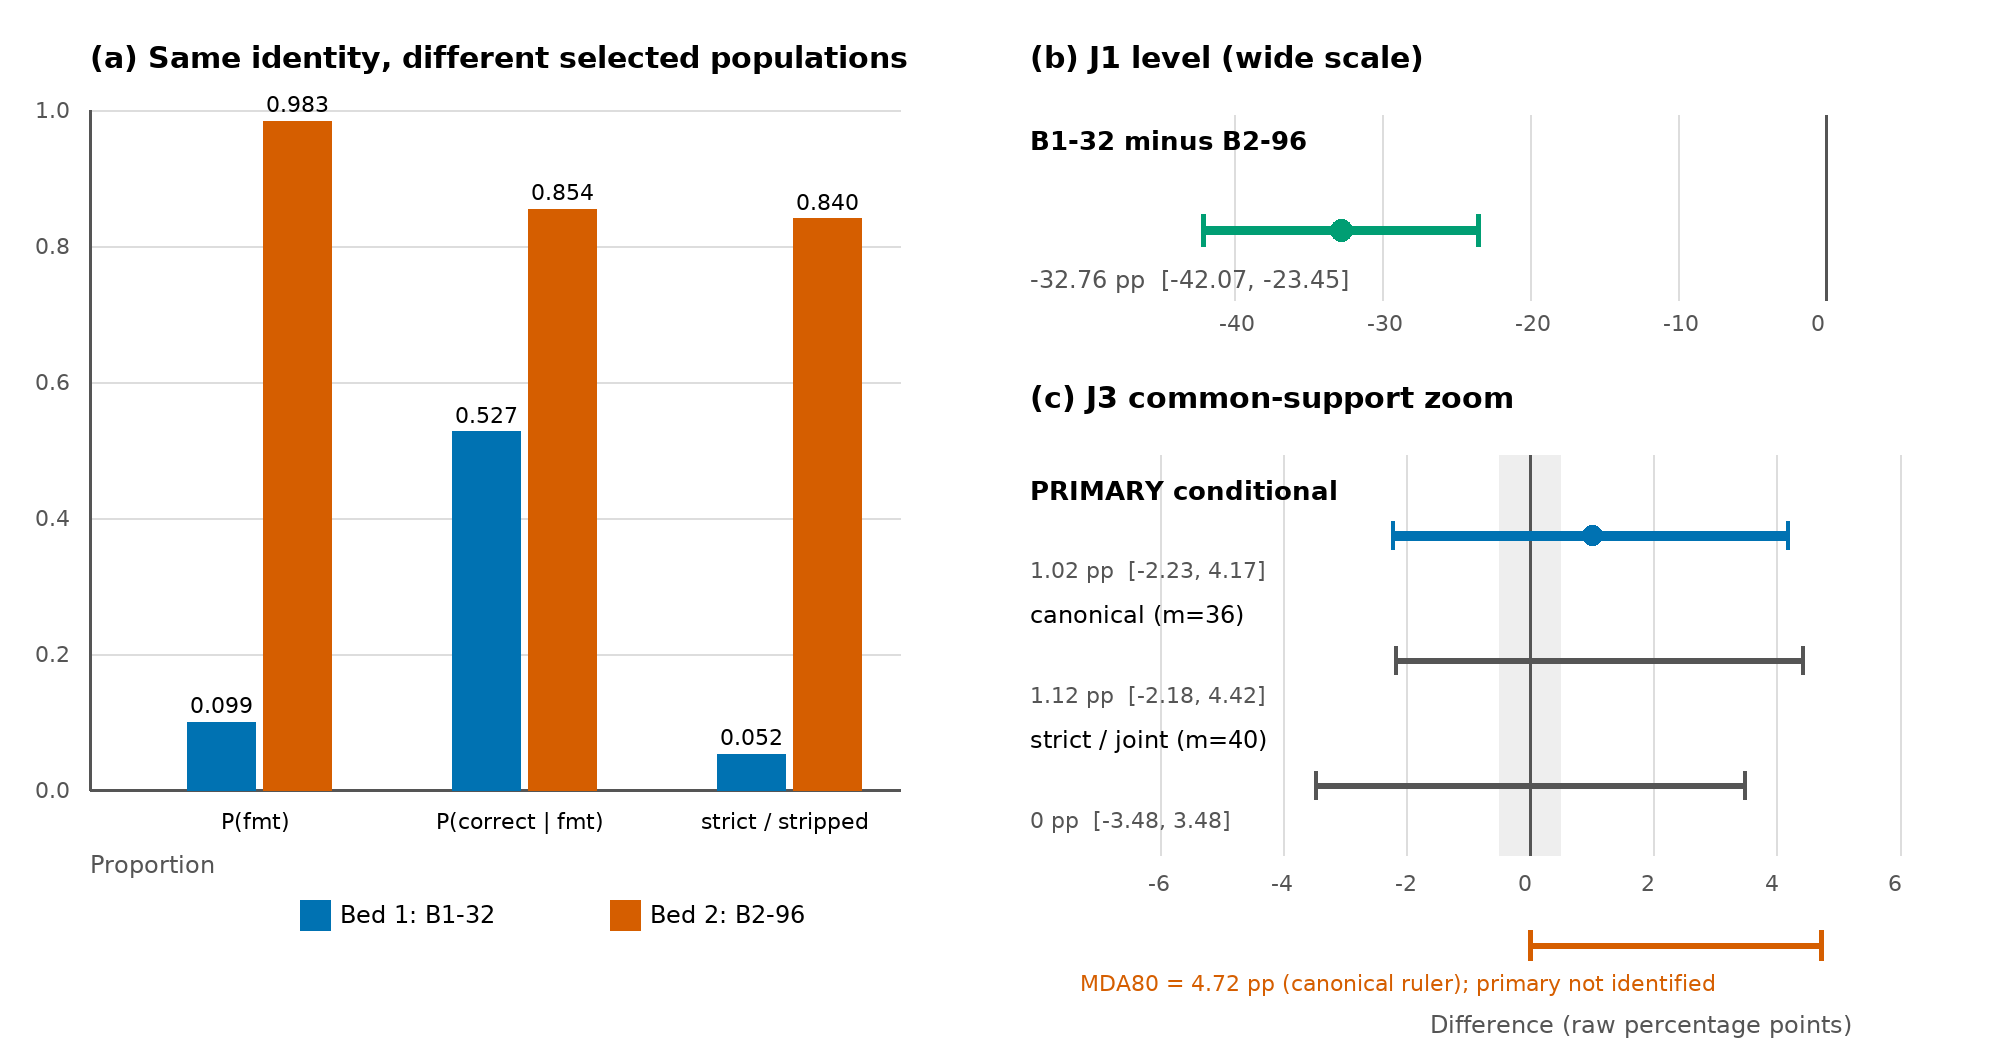
\includegraphics[width=\textwidth]{figures/judge_normalization_summary.png}
  \caption{\textbf{Machine-derived normalization summary.}
  (a) The same identity holds on both beds despite sharply different format
  coverage.  (b) J1 is shown on its own wide scale because it lacks a common
  selected population.  (c) The J3 zoom makes the \emph{primary conditional}
  estimand visually dominant; strict and canonical are secondary rulers.  The
  shaded $\pm0.5\pp$ explicitly post-hoc tolerance and the $4.72\pp$ canonical-ruler
  MDA80 bracket show why a point outside tolerance with an interval straddling
  zero is not identified as equivalent: the data cannot decide.  MDA80 for the
  primary conditional ruler is not identified from the shipped summaries; a
  retrospective, post-hoc normal approximation from its reported CI gives
  $\approx4.57\pp$, distinct from the secondary-ruler bracket.  Values
  come from the frozen per-item Bed~2 rerun and conditional paired analysis;
  the rendering script asserts their hashes.}
  \label{fig:summary}
\end{figure}

\begin{table*}[!tb]
\centering\footnotesize
\setlength{\tabcolsep}{3pt}
\begin{tabular}{@{}lrrrrr@{}}
\toprule
arm & $n_{\mathrm{fmt}}$ & $a{=}P(\mathrm{corr}\mid\mathrm{fmt})$ &
$P(\mathrm{corr}\mid\neg\mathrm{fmt})$ & $\Delta$ (pp) & $z$ (S1/S2) \\
\midrule
\textsc{B1-32} (J1) & 131 & 0.526718 & 0.450337 & $+7.64$ & 1.662 / 1.662 \\
\textsc{B1-64} & 149 & 0.664430 & 0.605983 & $+5.84$ & 1.417 / 1.417 \\
\textsc{B1-128} & 160 & 0.806250 & 0.723037 & $+8.32$ & 2.455 / 3.445 \\
\textsc{B1-256} & 348 & 0.824713 & 0.745623 & $+7.91$ & 3.200 / 4.254 \\
\textsc{B0-256} & 351 & 0.831909 & 0.742769 & $+8.91$ & 3.652 / 4.362 \\
\textsc{H-PRED-95} & 147 & 0.775510 & 0.709898 & $+6.56$ & 1.779 / 2.006 \\
\textsc{H-DAEDAL-1024} & 165 & 0.848485 & 0.758232 & $+9.03$ & 2.947 / 2.947 \\
\textsc{H-VAR} & 137 & 0.540146 & 0.445008 & $+9.51$ & 2.116 / 2.116 \\
\bottomrule
\end{tabular}
\caption{Per-channel classification accuracy on the eight reproducible Bed~1
arms (source: the per-arm accuracy table;
$n{=}1319$ items/arm;
$z$ uses the unpaired two-proportion formal interval).  The format
channel ($\mathrm{fmt}$) exceeds the fallback channel
($\neg\mathrm{fmt}$) on \emph{all eight} arms under S1 ($5.8$--$9.5\pp$; the
direction also holds on all eight under S2): five of the eight S1 differences
clear $z{=}1.96$ at $\alpha{=}0.05$
(\textsc{B1-128}, \textsc{B1-256}, \textsc{B0-256},
\textsc{H-DAEDAL-1024}, \textsc{H-VAR}), and six do under S2, which adds
\textsc{H-PRED-95}.  The final column reports every arm
under S1 (tight-correct, used by all paper computations) and S2
(raw-whitelist alternative), in that order.  At the Bonferroni boundary
$z{=}2.7339$, the tally is therefore a source range of $3$--$4/8$: 3 under S1
and 4 under S2.  \textsc{B1-128} crosses only under S2; its S1 $z{=}2.455$
lies between the uncorrected $1.96$ and Bonferroni $2.7339$ boundaries and
needs $+2$ flips ($+1.25\pp$ on $a_{\mathrm{fmt}}$) to cross.
The dual values are reproducible from
\protect\path{results/r428_dual_source_sweep.json} (validation against the frozen
\texttt{c3\_tight} accuracies at $10^{-5}$).  Four cells have a nonzero
S1-versus-S2 formatted-correct count---\textsc{B1-128}: 129 vs.\ 133;
\textsc{B1-256}: 287 vs.\ 293; \textsc{B0-256}: 292 vs.\ 296;
\textsc{H-PRED-95}: 114 vs.\ 115 (the first two are the reviewer-queried
pair)---and each is an item-level extractor-fidelity difference where the
canonical extractor rescued a correct answer the strict extractor refused;
the other four arms agree exactly, so their two $z$ values coincide.
Only \textsc{B1-128} changes Bonferroni status between sources.  For the
remaining sub-threshold S1 cells, \textsc{H-VAR} needs 4 flips;
\textsc{H-PRED-95} needs 5; \textsc{B1-32} needs 6; \textsc{B1-64} needs 7.
No other cell is within two flips of the boundary.
For \textsc{B1-32}, the displayed channel accuracies are
$69/131=0.527$ (formatted) and $535/1188=0.450$ (unformatted), while
Table~\ref{tab:rescue} reports the distinct $535/604=88.6\%$ rescue share.
The 8-for-8 direction tally is descriptive: the arms share the same 1,319-item
pool and generator, so it is not a claim of eight independent Bernoulli
replicates.  An item-clustered permutation would be the inferential form and is
not claimed here; bootstrap intervals and paired tests elsewhere cluster by
problem ID.  On the J1 arm alone the
difference is not significant ($z{=}1.66$).  The $88.6\%$ headline ratio
is driven by the low format-emission base rate ($q{=}0.0993$ on
\textsc{B1-32}), not by rescue being a noise source.}\label{tab:channels}
\end{table*}

Both channels classify many frozen items correctly, but the format channel is
consistently $5.8$--$9.5\pp$ higher ($5/8$ uncorrected-significant under S1 and
$6/8$ under S2; $3$--$4/8$ Bonferroni across the two frozen strict-cell sources;
Table~\ref{tab:channels}).  That modest directional gap is
real evidence against channel equivalence, yet it is far too small to explain
the $35$--$67\times$ rescue-share contrast.  The contrast is therefore
\emph{prevalence-dominated}: $q$ is low on Bed~1 and near one on Bed~2.  The
gate makes that distinction visible by requiring $q$, $a$, and $s$ together;
the strict ruler's treatment of all 535 rescued \textsc{B1-32} answers as
wrong is not a clean capability correction.

\subsection{J2: raw order first, with a disclosed paired-gate rule sensitivity}\label{sec:j2}

The estimand wording ``definite'' was pre-registered, but its criterion was
operationalized post hoc after inspecting the data, in the claim-preserving direction:
a canonical relation is definite only when exact two-sided McNemar has
$p<.05$ \emph{and} an item-paired bootstrap interval excludes zero.  This is a
directionally favorable rule sensitivity: the gate was pre-registered in
estimand wording and operationalized post hoc.  Pairing itself is appropriate
because every Bed~1 arm scores the same 1,319 items; the disclosure concerns
when and why the gate was chosen.  The full matrix uses $B=2000$ paired
resamples.  J3 uses $B=5000$ for its single primary interval; each count was
fixed in its analysis script before resampling, and the unequal computational
allocation carries no evidentiary ranking.

The exact McNemar $p$ values and the $p<.05$ eligibility rule are raw and
two-sided.  Dunn--Bonferroni family-wise control is reported as a separate
multiplicity sensitivity; it does not retrospectively redefine eligibility.

Accordingly J2 is reported as a raw-first rule-pair, not a unified
pre-registered verdict: the raw point-estimate rule reads $3/28$, while the
paired significance gate reads $F_{\mathrm{strip}}=0/23$ as a
favorable, post-hoc rule sensitivity; each looser definite gate has two
reversals.  Table~\ref{tab:j2-gates} keeps the non-interchangeable raw,
paired-definite, and planned-arm denominators together; the complete Bed~1
matrix is in Appendix~\ref{sec:appx_j2tab}.

\begin{table*}[!htbp]
\centering\footnotesize
\setlength{\tabcolsep}{2pt}
\begin{tabular}{@{}>{\raggedright\arraybackslash}p{2.8cm}
                    >{\centering\arraybackslash}p{1.25cm}
                    >{\centering\arraybackslash}p{1.45cm}
                    >{\raggedright\arraybackslash}p{1.8cm}
                    >{\raggedright\arraybackslash}p{6.05cm}@{}}
\toprule
Reading & Eligible & Reversals & Item-paired strata & Role / observed sensitivity \\
\midrule
Bed~1 raw sign & 28 & 3 & $3/4$, $0/4$, $0/20$ & Lead point-estimate rule; eight of nine arms identifiable. \\
Bed~1 paired canonical-definite & 23 & 0 & $0/3$, $0/20$ & Favorable rule sensitivity; estimand wording pre-registered, criterion operationalized post hoc. \\
Merged gate set & 25 & 0 & --- & Bed~1 gate plus two definite Bed~2 baseline pairs. \\
Bed~2 paired canonical-definite & 2 & 0 & --- & Power-limited inventory, derived in Table~\ref{tab:bed2-j2}. \\
Bed~1 strict-definite & 22 & 2 & --- & Looser definite gate; two reversals. \\
Bed~1 either-definite union & 25 & 2 & --- & Looser definite gate; the same two reversals. \\
Adversarial planned-arm bound & 31 gated / 36 raw & at most 8 / 11 & --- & Missing ninth arm assigned the reviewer-most-adverse plausible reversals. \\
\bottomrule
\end{tabular}
\caption{J2 rule-pair and looser gates.  The two looser-gate reversals are
\textsc{B1-256}--\textsc{H-DAEDAL-1024} and
\textsc{B0-256}--\textsc{H-DAEDAL-1024}, both canonical near-ties whose paired
intervals include zero; the raw rule adds a third near-tie.  Every zero here is
a descriptive count, not a probability: this revision withdraws the
independent-Bernoulli zero-event upper bounds this column previously carried,
because all pairs are built from the same shared problem IDs and are therefore
not independent trials (the withdrawn values are itemized in
Appendix~\ref{sec:appx_deviations}).  The replacement column reports the
item-paired $|\Delta_{\mathrm{can}}|$ strata of Table~\ref{tab:j2-diagnostics}
in the order ${<}1\pp$, $1$--${<}4\pp$, ${\geq}4\pp$, which localizes where the
reversals actually sit rather than converting a zero into confidence.  Exact
McNemar $p$ values and gate eligibility are raw and two-sided;
Dunn--Bonferroni family-wise control is a separate sensitivity.
The favorable paired gate---pre-registered in estimand wording and
operationalized post hoc---is near-collinear with the reversal mechanism: its
criterion conditions away the ambiguous near-ties where every observed raw
reversal occurs.}
\label{tab:j2-gates}
\end{table*}

The shipped Bed~1 records identify only eight arms (28 pairs), although the
frozen plan asserts nine arms (36 pairs); the ninth arm is unidentifiable from
the shipped records.  Under an adversarial assignment of plausible reversals,
the bound is $8/31$ on the gated support and $11/36$ on the raw 36-pair plan;
both denominators are carried in the last row of Table~\ref{tab:j2-gates}.

The gate is near-collinear with the reversal mechanism it conditions on:
definite-by-construction excludes the ambiguous pairs.  Table~\ref{tab:j2-diagnostics}
makes that conditioning visible and co-reports the frozen arm-resampling and
sharp sign-null diagnostics.  Every observed raw reversal lies in the
smallest-gap stratum removed by the paired gate; the gated zero is therefore a
conditional sensitivity reading, not evidence that raw order is universally
preserved.

\begin{table}[!t]
\centering\footnotesize
\setlength{\tabcolsep}{2pt}
\begin{tabular}{@{}>{\raggedright\arraybackslash}p{3.5cm}
                    >{\centering\arraybackslash}p{2.0cm}
                    >{\raggedright\arraybackslash}p{3.4cm}
                    >{\raggedright\arraybackslash}p{4.6cm}@{}}
\toprule
Diagnostic & Support & Result & Takeaway \\
\midrule
Raw gap $|\Delta_{\mathrm{can}}|<1\pp$ & 4 pairs & 3 reversals & All observed raw reversals are near-ties. \\
Raw gap $1\leq|\Delta_{\mathrm{can}}|<4\pp$ & 4 pairs & 0 reversals & No reversal in the middle stratum. \\
Raw gap $|\Delta_{\mathrm{can}}|\geq4\pp$ & 20 pairs & 0 reversals & No reversal in the widest-gap stratum. \\
Strict-channel arm permutation & 2{,}000 draws & $0$ draws with $F_{\mathrm{strip}}\geq1$ & Canonical pairing fixed; definite count clusters at 21--23. \\
Canonical-channel arm permutation & 2{,}000 draws & $0$ draws with $F_{\mathrm{strip}}\geq1$ & Strict pairing fixed; definite count clusters at 21--23. \\
Sharp sign exchangeability & 23 definite pairs & $P(F_{\mathrm{strip}}=0\mid H_0)=2^{-23}\approx1.2\!\times\!10^{-7}$ & Fair-coin diagnostic for each definite pair's strict sign. \\
\bottomrule
\end{tabular}
\caption{Gate-selection diagnostics for J2.  Gap rows stratify the frozen
28-pair raw matrix; null rows summarize the two single-channel arm-permutation
checks and the sharp sign-exchangeability calculation.  The permutation
script reproduces every arm's frozen canonical/strict accuracy to $10^{-5}$;
artifact paths are in Appendix~\ref{sec:appx_repro}.  These are null
diagnostics, not population reversal guarantees.  Within the favorable
paired-definite subset, no below-$1\pp$ pair is eligible; the two wider strata
contain $0/3$ and $0/20$ reversals.  All counts share problem IDs and are
descriptive rather than independent-Bernoulli probability statements.}
\label{tab:j2-diagnostics}
\end{table}

The complete Bed~2 denominator is derived item by item in
Table~\ref{tab:bed2-j2}: four fixed-128 baseline contrasts are pairable, two
are non-definite, and therefore eligible $=4-0-2=2$.

Thus the evidence is deliberately dual: three reversals among all 28 raw signs,
but none among 23 definite Bed~1 pairs under the paired gate that was
pre-registered in estimand wording, operationalized post hoc, and favorable in
direction; Bed~2's
two-pair definite inventory is too small to support a broad zero-reversal law.

\subsection{J3: the registered tie, recomputed on common support}\label{sec:j3}

The full-pool canonical tie is an artifact of comparing supports of different
sizes.  We therefore align \textsc{B2-128} and \textsc{B2-160} on the common over-half and
report the strict, canonical, and conditional rulers separately in
Table~\ref{tab:j3-estimands}.

The strict row is a genuine exact tie but remains auxiliary: the
preregistration assigns J3 to the primary conditional ruler.  The canonical
row is fallback-inclusive over all common-support items, not conditional on
format.  Direct enumeration of the frozen per-item Bed~2 rerun resolves the
unformatted B2-128 count as $u{=}5$ (previously $u\in\{4,5\}$), producing the conditional row rather
than collapsing distinct rulers into one number.  The exact fields and artifact
hash appear in Appendix~\ref{sec:appx_artifact}; the same records support the
conditional paired
bootstrap.

The registered primary point estimate crosses the explicitly post-hoc center
tolerance, but its
paired interval contains zero and the detectable resolution reported in the
caption is much coarser.  J3 is therefore \textsc{not\_identified} from the
shipped summaries: the data cannot decide, and failing to reject the null is
not proof of no effect.  We neither claim a broken tie nor retain the exact-tie
label.  The old
full-sample result conflated the rulers and populations and is retracted in
\S\ref{sec:deviations}.  As always, an interval containing zero is not evidence
of equivalence; resolving the post-hoc tolerance would require a much larger
paired sample.

\begin{table}[!t]
\centering\footnotesize
\setlength{\tabcolsep}{2pt}
\begin{tabular}{@{}>{\raggedright\arraybackslash}p{2.0cm}
                    >{\raggedright\arraybackslash}p{2.4cm}
                    >{\raggedright\arraybackslash}p{2.4cm}
                    >{\raggedright\arraybackslash}p{1.35cm}
                    >{\raggedright\arraybackslash}p{5.15cm}@{}}
\toprule
Ruler & \textsc{B2-128} & \textsc{B2-160} & $\Delta$ (pp) & Paired evidence and role \\
\midrule
Strict / joint $s$ & $310/356=0.8708$ & $310/356=0.8708$ & $0.00$ &
$m{=}40$, $p{=}1$, CI $[-3.48,3.48]$; exact tie, auxiliary. \\
Canonical & $314/356=0.8820$ & $318/356=0.8933$ & $+1.12$ &
$m{=}36$, $p{=}0.6177$, CI $[-2.18,4.42]$; fallback-inclusive sensitivity. \\
Conditional $\PcFmt$ & $310/351=0.8832$ & $310/347=0.8934$ & $+1.018$ &
Item-paired bootstrap CI $[-2.23,+4.17]$ ($B{=}5000$); primary marginal
conditional estimand, not identified from the shipped summaries.  Equal
numerators ($310=310$) make this gap entirely a four-item denominator effect. \\
Joint-format sensitivity & $304/342=0.8889$ & $306/342=0.8947$ & $+0.585$ &
Both-formatted support; McNemar $m{=}30$, $p{=}0.8555$. \\
Superseded conditional mixed support & --- & --- & $+0.08$ &
CI $[-4.06,3.90]$; re-signed to the current $a_{160}-a_{128}$ convention;
source fractions omitted because the populations differ. \\
\bottomrule
\end{tabular}
\caption{J3 estimands after support alignment.  The superseded mixed-support
row is retained only for provenance and re-signed from the legacy
$a_{128}-a_{160}$ convention to the current $a_{160}-a_{128}$ convention; its
source fractions ($623/698$ vs.\ $310/347$) remain in
Appendix~\ref{sec:appx_artifact} because the
populations differ.  The auxiliary strict ruler ties exactly, whereas the
registered primary conditional gap is $+1.018\pp$ with a paired interval that
contains zero; its equal numerators ($310=310$) are a frozen-data coincidence,
and the gap is a four-item denominator effect ($351$ vs.\ $347$ after resolving
$u{=}5$).  Canonical/strict MDA80 values are $4.719/4.977\pp$; primary
conditional MDA80 is not identified from the shipped summaries.  A
retrospective, post-hoc normal approximation from the conditional CI half-width
gives $2.802(3.20/1.96)\approx4.57\pp$; it is a CI-derived resolution, not a
shipped or preregistered MDA80.  The arm-wise conditional point estimates
($310/351$ and $310/347$) and the joint McNemar support ($n=342$) are different
subsets.  The $+1.018\pp$ arm-wise gap is entirely a denominator effect because
the numerators are equal ($310=310$); the $n=342$ intersection supports the
separate joint-format test.  At $n_{\mathrm{selected}}=347$, two
flips drop the point below the explicitly post-hoc $0.5\pp$ tolerance, four
reduce it to zero, and eight lift the 95\% CI lower bound above zero
(\protect\path{results/r428_j3_oneflip.json}).  Thus the primary result remains
\textsc{not\_identified} from the shipped summaries---the data cannot
decide---not an equivalence or robustness-to-zero claim.
Paired bootstrap and exact-test units are problem IDs whenever records share
question identifiers.}
\label{tab:j3-estimands}
\end{table}

\subsection{Deviations from the preregistration}\label{sec:deviations}

Appendix~\ref{sec:appx_deviations} itemizes every departure from the pre-data
record, including the J3 population/estimand, the order gate whose wording was
pre-registered but criterion operationalized post hoc, the J1 capability
reading, and the synthesis operationalized post hoc, with each directional
effect.

\paragraph{A hierarchy of two-bed claims.}
The evidence supports a hierarchy, not a binary ``comparable / not
comparable'' verdict; Tables~\ref{tab:judgments},
\ref{tab:interpretation-checklist}, and
\ref{tab:interpretation-checklist-continued} carry every value quoted in this
paragraph beside the result it qualifies.  A level claim needs a common scale
and common selected
population; neither is available.  The raw order rule has three reversals among
28 pairs, while the favorable paired-gate rule sensitivity---pre-registered
in estimand wording and operationalized post hoc---has no definite reversal
among 23
pairs.  A pattern claim asks whether a registered tie changes its label;
on the pre-registered primary estimand J3 is \textsc{not\_identified} from the
shipped summaries---the data cannot decide: its
$+1.02\pp$ conditional gap exceeds the explicitly post-hoc $0.5\pp$ tolerance,
but the item-paired
$95\%$ CI contains zero, so the data cannot decide---while an exact tie
persists only under the auxiliary strict estimand.  MDA80 for the primary
conditional ruler is not identified; the canonical/strict secondary rulers
have resolutions of $4.719/4.977\pp$, while the primary conditional CI gives
only a retrospective, post-hoc $\approx4.57\pp$ resolution.  The hierarchy
therefore co-reports the favorable gated zero with raw and looser-gate
reversals; it does not promote that zero into a universal order law.

\begin{table*}[!h]
\centering\footnotesize
\setlength{\tabcolsep}{3pt}
\begin{tabular}{@{}>{\raggedright\arraybackslash}p{0.8cm}
                    >{\raggedright\arraybackslash}p{2.9cm}
                    >{\raggedright\arraybackslash}p{4.60cm}
                    >{\raggedright\arraybackslash}p{5.05cm}@{}}
\toprule
ID & Question & Frozen observation & Decision and scope \\
\midrule
J1 & Two-bed level after conditioning &
$-32.76\pp$, CI $[-42.07,-23.45]$; $q=0.0993$ vs. $0.9831$; design-entailed &
\blocked: non-common selected populations plus task confounding. \\
Joint & Fallback-stripped level &
$-78.76\pp$, CI $[-82.75,-74.76]$; additive share $[59.11\%,95.87\%]$; log share $82.58\%$ &
Additive point attribution is not identified; log is anchor-free and exact for positive multiplicative factors. \\
J2 & \emph{Definite} order reversal &
Bed~1: $3/28$ raw, $0/23$ disclosed paired, and $2$ under both looser gates; Bed~2: $0/2$ &
Raw-first rule-pair; the favorable paired gate was pre-registered in estimand
wording but operationalized post hoc.  Descriptive raw strata are $3/4$ below
$1\pp$, $0/4$ at $1$--$<4\pp$, and $0/20$ at $\geq4\pp$; shared problem IDs
preclude an independent-Bernoulli probability reading. \\
J3 & Registered tie after normalization (common support) &
strict tie ($310=310$, $m{=}40$, $p{=}1$); canonical $+1.12\pp$; primary marginal conditional $+1.018\pp$, joint-format $+0.585\pp$ &
Primary \textsc{not\_identified} from the shipped summaries: the data cannot
decide because CI $[-2.23,+4.17]\pp$ contains zero.  Primary MDA80 is not
identified; canonical/strict secondary values are $4.719/4.977\pp$, and the
primary CI-derived post-hoc resolution is $\approx4.57\pp$.  Strict tie is
auxiliary; no TOST. \\
Final & Synthesis &
J1 level blocked; J2 is rule-dependent; J3 tie not identified on its primary estimand &
Pre-registered in estimand wording, operationalized post hoc as a hierarchy:
the raw rule has reversals while the favorable paired gate reads zero; pattern
is not identified from the shipped summaries and level is inadmissible. \\
\bottomrule
\end{tabular}
\caption{Decision audit, distinguishing pre-registered elements from post-hoc
revisions. Effects use raw pp; Add./Log. are defined in \S\ref{sec:results}.}
\label{tab:judgments}
\end{table*}

\paragraph{The gate.}\label{sec:gate}
For any conclusion whose canonical score can use fallback: (i) report $\Pfmt$,
$\PcFmt$, and their joint product; (ii) state formatted-subset coverage on every
bed; (iii) retest the relation after fallback removal; and (iv) reject a
two-bed level law unless common support and task-scale comparability are
separately justified.
Passing the gate permits only the relation actually tested.  It never upgrades
an observed zero reversal into a universal law.

\section{Limitations and validity threats}
\label{sec:limitations}

This audit spans only two beds, two rulers, and different tasks/prompts.
$\PcFmt$ conditions on arm-varying post-outcome (post-generation) behavior, so level contrasts
are descriptive; unregistered reweighting is unavailable.  Unpaired claims
use normal intervals; J3 uses the paired common support.  Only two Bed~2 J2
pairs are definite, and J3 cannot resolve the post-hoc $0.5\pp$ tolerance.
Whitelist-strict behavior
is partly constructional, but formatted-row errors remain data-dependent and
need retesting.  No pooled two-bed SD exists; pp effects are unstandardized.

\paragraph{Reproducibility statement.}\label{sec:repro}
Appendix~\ref{sec:appx_artifact} lists exact fields and SHA anchors, interval
conventions, the
numeric guard, and deterministic build.  Analysis is reproducible from the
shipped tables, while generation inherits the frozen-trial disclosure: seeds
and temperatures absent from those records cannot be reconstructed.  The
canonical-item rebuild verification and its below-gate drift record are frozen
alongside the artifact; Appendix~\ref{sec:appx_repro} gives the role-named
paths and exact fidelity result.

\subsection{Positioning against the external calibration review}
An external calibration review of this manuscript returned soundness~3,
contribution~2, presentation~5, and overall~3 (clear reject) with no fatal
issue.  That grade, not the more favorable internal panel, is the anchor we
position against, and we state its central objection without softening it: the
contribution is judged incremental because $s=qa$ is a probability identity,
Wilson/McNemar/bootstrap are standard tools, and---decisively---the nearest
extraction work is cited rather than compared on the same bed.  We do not claim
to have closed that gap.  Appendix~\ref{sec:appx_parser} narrows it only to the
extent a zero-GPU reparse can: it compares the anchor-first xFinder regex tier
on both frozen beds, leaving the learned tier, Answer Regeneration, and any
human-adjudicated gold standard explicitly unattempted, and
Table~\ref{tab:closest-work} marks that boundary component by component.
Raising contribution therefore requires the multi-parser, human-adjudicated,
multi-model experiment named in that review, which is outside this revision's
zero-GPU budget.  The reviewer's requested channel-precision
view is likewise bounded: it is the deterministic reference-match audit in
Tables~\ref{tab:channels} and~\ref{tab:strict-reconciliation}, which is a
parser-precision \emph{proxy} on the shipped items and not a substitute for new
human labels.  Its five most visible objections map to body-level
dispositions: \emph{(i)} J1 is declared inadmissible as a capability comparison
because of non-common selected populations and task confounding
(\S\ref{sec:results}), not ``proven'' away; \emph{(ii)} J2 is a two-bed-scoped
rule-pair---raw $3/28$, favorable paired $0/23$ with a gate pre-registered in
estimand wording but operationalized post hoc, and two reversals under each
looser gate---rather than an order-preservation law (\S\ref{sec:j2});
\emph{(iii)} J3 is \textsc{not\_identified} from the shipped summaries---the
data cannot decide, its CI contains zero, and no TOST is claimed---with all
three MDA rulers separated in Table~\ref{tab:j3-estimands}; \emph{(iv)} the
Bed-qualified \textsc{B2-*} convention resolves the cross-bed name collision
(Table~\ref{tab:vocabulary}); and \emph{(v)} the parser is a deterministic
string matcher, not an LLM judge, as distinguished in \S\ref{sec:related} and
Appendix~\ref{sec:appx_parser}.  These are pointers to the zero-GPU
reconciliation already reported, not a defense by re-argument.

\paragraph{Ethics statement.} No human participants or personal data are
used.  The main risk---misleading capability comparison---is addressed by
scoped claims, post-hoc operationalization labels, and provenance.

\section{Conclusion}
\label{sec:conclusion}

Fallback removal is necessary but insufficient.  The format channel has a
modest directional advantage, but it is far too small to explain the
prevalence-dominated rescue-ratio contrast (Table~\ref{tab:channels}).  The
order result is rule-dependent: the raw-first and disclosed paired-gate
readings differ; the paired gate is favorable, pre-registered in estimand
wording, and operationalized post hoc (Table~\ref{tab:j2-gates}).  J3 is
\textsc{not\_identified} from the shipped summaries---the data cannot
decide---on its primary conditional estimand, and J1 is descriptive, not a capability law
(Tables~\ref{tab:j3-estimands} and~\ref{tab:judgments}).  The additive
attribution is not identified, its legal range contains the unique log share,
and no scale discrepancy is claimed (Table~\ref{tab:j1-decomposition}).
Reporting $q$, $a$, and $s=qa$ exposes these boundaries.

\bibliographystyle{iclr2026_conference}
% P5_MAIN_TEXT_END
\label{p5:main-text-end}
\bibliography{refs}

\paragraph{AI assistance disclosure.}
AI-assisted writing and image-generation tools were used to reorganize,
typeset, and check this manuscript and to produce the conceptual Figure~1.
All numerical claims and Figure~2 were restricted to the frozen machine
artifact and mapped to explicit evidence IDs; no experiment or citation was
created by the writing tool.

\appendix
\raggedbottom

\paragraph{Appendix roadmap.}
The appendices are ordered by role rather than by order of citation, because the
main text reaches the parser and deviation ledgers before it needs the provenance
manifest.  Appendix~\ref{sec:appx_artifact} is the artifact manifest and
availability statement (including the per-claim provenance and strict-cell
reconciliation tables); Appendix~\ref{sec:appx_supporting} holds the supporting
numeric audits; Appendix~\ref{sec:appx_j2tab} is the complete J2 paired
definiteness inventory; Appendix~\ref{sec:appx_parser} is the same-bed
parser-lineage audit; and Appendix~\ref{sec:appx_deviations} is the full
deviation list.  Every appendix letter in this paper is resolved by the
compiler from its label, so no cross-reference depends on a hand-written letter.

\section{Artifact manifest}\label{sec:appx_artifact}
\label{app:artifact-manifest}

The current quantitative evidence is
\path{results/judge_normalization/judgment_table.json}, SHA-256 prefix
\texttt{c77ec165} (J-value set frozen as \texttt{566a1983c268}); the
preregistration SHA-256 prefix is \texttt{974d687224b1}; full hashes are
recorded in \path{evidence/repository_inventory.md} and the build audit.
The analysis script, data-figure script, claim map, and method map are,
respectively, \texttt{scripts/judge\_normalization.py},
\texttt{scripts/plot\_judge\_normalization.py},
\texttt{evidence/claim\_evidence\_map.tsv}, and
\texttt{evidence/method\_provenance.tsv}.  The data-figure script asserts the
evidence hash before rendering.

\subsection{Availability and reproducibility}
\label{sec:appx_repro}

{\raggedright
An anonymized supplementary artifact bundle accompanies the submission.  Its
manifest pointer is \path{paper/.p5_iclr_manifest.json}, whose SHA-256 is
\texttt{a76a7071d0ce6e6a4ec6ea72c89338eb45051e0847bfe57dccaa487ace71d508};
the official-template archive recorded inside it has SHA-256
\texttt{b6d63b29992e153f804bb6d170c57db156c011b5bedf96a9f31d58813b909acf}.
Analysis is fully reproducible from the shipped tables and scripts.  Generation
is only reproducible to the extent certified by the frozen trial artifacts:
model, split, arm budgets, and outputs are present, while missing sampling seeds
and temperatures are disclosed rather than reconstructed.\par}

{\raggedright
\textbf{Availability.} The anonymized supplementary bundle, the build ledger,
the canonical-items rebuild verification scripts
(\texttt{scripts/r419\_parser\_lab/parsers.py},
\texttt{scripts/r419\_parser\_lab/run\_lab.py}), the numeric-guard script
(\texttt{scripts/check\_numeric\_tables.py}) together with its recorded output
(\texttt{results/r409\_numeric\_table\_guard.json}), and the Figure~2 renderer
are frozen with the artifact and are listed by role in the remainder of this
subsection.  Frozen trial artifacts are not redistributed;
their role-named identifiers suffice to re-derive the numeric claims from the
shipped tables alone.  Consolidated role pointers are: the bundle and build
ledger in this Availability paragraph; canonical parser rebuild, numeric-guard,
and Figure~2 renderer paths immediately below; and the irrecoverable
seed/temperature disclosure in \S\ref{sec:beds} and \S\ref{sec:repro}.\par}

The canonical-items rebuild verification assets are
\path{scripts/r419_parser_lab/parsers.py} and
\path{scripts/r419_parser_lab/run_lab.py}, with evidence in
\path{results/r419_parser_lab/lab_results.json}.  They record canonical-extractor
drift $6/2136=0.28\%$, below the pre-registered $2\%$ gate in
\texttt{prereg/\allowbreak R419\_PREREG\_\allowbreak SAMEBED\_\allowbreak
NEAREST\_\allowbreak NEIGHBOR\_\allowbreak REPARSE.md}.

\paragraph{Shipped assertion suite.}
The cell-level numeric guard is \path{scripts/check_numeric_tables.py} with its
recorded output \path{results/r409_numeric_table_guard.json}.  The Figure~2
renderer asserts that the $4.719\pp$ and $4.977\pp$ MDA80 fields retain their
canonical/strict ruler labels and that the primary conditional ruler is not
assigned either value.  The primary conditional CI-derived
$\approx4.57\pp$ resolution is explicitly post-hoc and is not asserted as a
shipped MDA80.  The denominator-convention assets are the frozen J2
rule file and paired result; together they assert 28 raw pairs, 23 gated pairs,
and the separately derived ninth-arm bounds.  These are descriptions of shipped
checks, not claims that new experimental runs were executed in this revision.

{\raggedright
The refine-6 J2 resampling-null assets are
\path{scripts/r427_fstrip_resampling_null.py},
\path{results/r427_fstrip_arm_resampling.json}, and
\path{results/r427_fstrip_nulls_supplement.json}; the script reconstructs every
frozen arm before applying the recorded single-channel permutations.\par}

\begin{table}[H]
\centering\footnotesize
\setlength{\tabcolsep}{3pt}
\begin{tabularx}{\columnwidth}{@{}>{\raggedright\arraybackslash}p{3.1cm}
                                  >{\raggedright\arraybackslash}p{3.2cm}
                                  >{\raggedright\arraybackslash}X@{}}
\toprule
Entry & Verified primary locator & Verification basis \\
\midrule
Dream 7B \citep{ye2025dream} & arXiv:2508.15487 & primary arXiv record, 2026-08-24 \\
Fast-dLLM \citep{wu2025fastdllm} & arXiv:2505.22618 & primary arXiv record, 2026-08-24 \\
Fast-dLLM v2 \citep{wu2025fastdllmv2} & arXiv:2509.26328 & primary arXiv record, 2026-08-24 \\
DreamOn \citep{wu2026dreamon} & arXiv:2602.01326 & primary arXiv record, 2026-08-24 \\
Jo et al. \citep{jo2025finding} & arXiv:2510.14773 & primary arXiv record, 2026-08-24 \\
xFinder \citep{yu2024xfinder} & arXiv:2405.11874 & primary arXiv record, 2026-08-24 \\
Selective classification \citep{elyaniv2010selective} & JMLR 11:1605--1641 & publisher record, 2026-08-24 \\
\bottomrule
\end{tabularx}
\caption{Completion of the per-entry verification ledger: the four previously
unlogged dLLM references and the positioning-critical Jo et al. entry.  The
remaining methodology entries are covered by the bounded retrieval ledger.}
\label{tab:reference-ledger}
\end{table}

{\raggedright
All $95\%$ confidence intervals use $z{=}1.96$ and one shared routine
(\texttt{scripts/judge\_normalization.py diff\_ci}; Wilson intervals via
\texttt{plot\_judge\_normalization.py}); endpoints are rounded half-up, and
full-precision values are stored in the frozen judgment table and the
per-item Bed~2 rerun \texttt{rebuild\_full.json} \path{paired_stats}.  The
original generation-and-judge references used
here \citep{cobbe2021gsm8k,nie2025llada,li2025daedal,zhou2026dllm,zheng2023judging}
were each verified against a primary arXiv record or an in-run multi-reviewer
citation ledger before inclusion; Table~\ref{tab:reference-ledger} records the
per-entry locator and verification basis for the entries that ledger had not
yet covered.  The eight methodology entries added in the
bounded positioning pass are independently fetch-verified in
\texttt{refs\_retrieval/r409\_refpos\_citations\_verify.json}.  Unverified
fields and failed retrievals are omitted rather than inferred from memory.\par}

\paragraph{Per-claim provenance.}
Each quantitative claim below resolves to one artifact, its SHA-256 prefix, and
the exact JSON field from which the value is read; every value is regenerated
in-repo (see \texttt{scripts/judge\_normalization.py} and
\texttt{scripts/plot\_judge\_normalization.py}).  Independent verification is
recorded in \path{results/r197_refine_verify/REFINE_VERIFY_R197.json}
(SHA-256 prefix \texttt{515a497a}).

The three independent provenance artifacts are named descriptively: the
per-arm accuracy table (\texttt{c3\_tight}), the frozen strict-decomposition
cells (\texttt{strict\_fmt\_decomposition}), and the per-item Bed~2 rerun
(\texttt{rebuild\_full.json}, SHA-256 prefix \texttt{bfebbed1}).
Their exact addresses are in \texttt{evidence/repository\_inventory.md}.

Table~\ref{tab:claim-provenance} maps each headline decision to its artifact,
hash prefix, and machine field.

\begin{table*}[!h]\centering\footnotesize
\setlength{\tabcolsep}{2pt}
\renewcommand{\arraystretch}{1.2}
\begin{tabular}{@{}>{\raggedright\arraybackslash\hyphenpenalty=10000}p{1.6cm}
                    >{\raggedright\arraybackslash}p{3.85cm}
                    >{\raggedright\arraybackslash}p{4.4cm}
                    >{\raggedright\arraybackslash}p{3.6cm}@{}}
\toprule
Claim & Artifact (SHA prefix) & JSON field path & Value \\
\midrule
Headline & \texttt{REFINE\_VERIFY\_R197} (\texttt{515a497a}) &
  \path{R1_headline/canon_correct}; \path{flip_rescued};
  \path{rescue_rate_pct}; \path{ratio_range_x} & $535/604=88.58\%$; $35.2$--$67.1\times$ \\
J1 level & \texttt{judgment\_table.json} (frozen \texttt{566a1983}, current \texttt{c77ec165}) &
  \texttt{J1\_\allowbreak crossbed\_\allowbreak level\_\allowbreak after\_normalize} & $\Delta=-32.76$ pp \\
J2 rule-pair & r402 paired analysis (\texttt{1fb1a156}) &
  \path{definite_paired_count}; \path{F_strip_definite_reversal};
  \path{F_strip_raw_reversal}; \path{n_pairs} & $0/23$ paired; $3/28$ raw \\
J3 strict & \texttt{rebuild\_full.json} (\texttt{bfebbed1}) &
  \texttt{paired\_\allowbreak stats/\allowbreak arm\_160\_strict} & $310$/$356$ m40 p1 \\
J3 canonical & \texttt{rebuild\_full.json} (\texttt{bfebbed1}) &
  \texttt{paired\_\allowbreak stats/\allowbreak arm\_160\_canonical} & $314/356$ vs. $318/356$; $+1.12$ pp \\
J3 primary conditional & r402 conditional-paired JSON (\texttt{17ec0132}) &
  \texttt{conditional\_estimand}; \texttt{paired\_bootstrap/ci95\_pp} & $310/351$ vs. $310/347$; $+1.018$ pp; $[-2.23,4.17]$ \\
J3 MDA rulers & r402 conditional paired + judgment table
  (\texttt{17ec0132}/\texttt{c77ec165}) &
  \texttt{paired\_bootstrap/ci95\_pp}; canonical/strict stored fields &
  primary MDA80 not identified; canonical/strict $4.719/4.977$ pp;
  post-hoc CI-derived primary resolution $\approx4.57$ pp \\
J3 joint-format & same conditional-paired JSON (\texttt{17ec0132}) &
  \texttt{both\_fmt\_mcnemar} & $304/342$ vs. $306/342$; $+0.585$ pp; $p=0.8555$ \\
J3 superseded & r409 Table-6 verification JSON (\texttt{60d5b441}) &
  \path{table6_superseded_row/true_source_recovered} & stored old-order $-0.082$ pp; current convention $+0.082$ pp \\
\bottomrule
\end{tabular}
\caption{Per-claim provenance for the headline values and decision audit.}
\label{tab:claim-provenance}
\end{table*}

The frozen \texttt{566a1983c268} judgment table remains the source for the J1
level claim, but its \texttt{J3\_equiv\_to\_sig\_is\_artifact} field (the old
$-0.08$\,pp full-sample value) is \textbf{superseded} for the J3 claim by the
per-item rerun's \texttt{paired\_stats/arm\_160\_\{strict,canonical\}}
common-support values and the conditional paired analysis
(see \S\ref{sec:j3} and J3 source notes), and its \texttt{J2} strict-pairs
inventory is superseded by \texttt{R197 R2\_J2\_8arm\_sensitivity} (28
reproducible pairs, 9th arm unidentified, as disclosed in
\S\ref{sec:deviations}).  The r402 paired artifacts govern the current J2 gate
and J3 primary interval; the per-item rerun governs the common-support counts.

Table~\ref{tab:strict-reconciliation} reconciles the strict molecules behind
the Headline row.  The two cited sources are the per-arm
\texttt{c3\_tight} table and the frozen
\texttt{strict\_fmt\_decomposition} cells.
The authoritative dual-source manifest is
\path{results/r428_dual_source_sweep.json} (SHA-256 prefix
\texttt{5d6f918c}): \path{rows[]/{source,n_fmt,fmt_correct,notfmt_correct,z}}
stores every displayed channel value, while
\path{construction/{S1_def,S2_def}} fixes S1 as tight-correct and S2 as the
raw-whitelist alternative.

\begin{table}[H]
\centering\footnotesize
\setlength{\tabcolsep}{3pt}
\begin{tabular}{@{}>{\raggedright\arraybackslash}p{3.0cm}
                    >{\raggedright\arraybackslash}p{3.0cm}
                    >{\raggedright\arraybackslash}p{3.0cm}
                    >{\raggedright\arraybackslash}p{4.2cm}@{}}
\toprule
Check & S1: per-arm \texttt{c3\_tight} & S2: frozen raw-whitelist & Consequence \\
\midrule
32/64-token, \textsc{H-DAEDAL-1024}, \textsc{H-VAR} cells & agree & agree & No source sensitivity; identical $z$. \\
\textsc{B1-128} $(n_{\rm fmt},\mathrm{correct})$ & $(160,129)$; $129/160$ & $(160,133)$; $133/160$ & Difference of 4 formatted-correct items. \\
\textsc{B1-256} $(n_{\rm fmt},\mathrm{correct})$ & $(348,287)$; $287/348$ & $(348,293)$; $293/348$ & Difference of 6 formatted-correct items. \\
\textsc{B0-256} $(n_{\rm fmt},\mathrm{correct})$ & $(351,292)$; $292/351$ & $(351,296)$; $296/351$ & Difference of 4 items; above the boundary under both sources. \\
\textsc{H-PRED-95} $(n_{\rm fmt},\mathrm{correct})$ & $(147,114)$; $114/147$ & $(147,115)$; $115/147$ & Difference of 1 item; below the boundary under both sources. \\
\textsc{B1-256} strict accuracy over all items & $287/1319=0.2176$ & $293/1319=0.2221$ & Source-to-column assignment matches the item row above. \\
Table~\ref{tab:channels} $z$ & B1-128: 2.455; B1-256: 3.200; B0-256: 3.652; H-PRED-95: 1.779 & B1-128: 3.445; B1-256: 4.254; B0-256: 4.362; H-PRED-95: 2.006 & Bonferroni count is $3/8$ (S1) versus $4/8$ (S2); only B1-128 switches. \\
\bottomrule
\end{tabular}
\caption{Strict-cell source reconciliation.  The r420 audit identified, and
this revision fixes, the prior
293/287 cross-column transposition.  S1 is always the per-arm tight-correct
source used by the paper's computations; S2 is the frozen raw-whitelist
alternative.  The integer pairs and all-item accuracies make that assignment
explicit rather than inferential.  The \textsc{B1-256}/\textsc{B0-256}
crossing is a \emph{between-source} point flip and not one of the $3/28$
canonical-versus-strict ruler reversals: within either source
\textsc{B0-256} stays higher ($0.2214$ vs.\ $0.2176$ under S1; $0.2244$ vs.\
$0.2221$ under S2), and the ordering flips only if a reader mixes
\textsc{B1-256} from S2 with \textsc{B0-256} from S1.  The order rule-pair is
unchanged, but the channel-wise Bonferroni count is the source range
$3$--$4/8$ shown for all eight arms in Table~\ref{tab:channels}.}
\label{tab:strict-reconciliation}
\end{table}

Our earlier wording (``No number in the body depends on those molecules'') was
too strong: Table~\ref{tab:channels} does depend on those cells.  All J2/J3
calculations in this paper take the per-arm \texttt{c3\_tight} values.

\section{Supporting numeric audits}\label{sec:appx_supporting}

\begin{table}[H]
\centering\footnotesize
\setlength{\tabcolsep}{2pt}
\begin{tabular}{@{}>{\raggedright\arraybackslash}p{1.8cm}
                    >{\centering\arraybackslash}p{1.45cm}
                    >{\centering\arraybackslash}p{1.45cm}
                    >{\centering\arraybackslash}p{1.45cm}
                    >{\centering\arraybackslash}p{2.5cm}
                    >{\centering\arraybackslash}p{1.9cm}
                    >{\centering\arraybackslash}p{1.6cm}@{}}
\toprule
Arm / contrast & $q$ & $a$ & $s=qa$ & Additive-share range & Symmetric share & Log share \\
\midrule
\textsc{B1-32} & $0.09931$ & $0.52672$ & $0.05232$ & --- & --- & --- \\
\textsc{B2-96} & $0.98315$ & $0.85428$ & $0.83991$ & --- & --- & --- \\
B1 minus B2 & $-0.88384$ & $-0.32756$ & $-0.78760$ & $[59.11\%,95.87\%]$ & $77.49\%$ & \textbf{$82.58\%$} \\
\bottomrule
\end{tabular}
\caption{J1 per-arm co-report and decomposition.  The first three columns are
the frozen format coverage, conditional accuracy, and exact product.  Every
additive split of $\Delta s$ requires an anchor: the two one-anchor rules span
$[59.11\%,95.87\%]$, so the additive share is not identified.  The symmetric
Oaxaca choice uses $\bar a=0.69050$, $\bar q=0.54123$, and
$\Delta s=\bar a\Delta q+\bar q\Delta a$; it is one sensitivity anchor.  The
primary anchor-free exact decomposition is
$\Delta\ln s=\Delta\ln q+\Delta\ln a$, with log share $82.58\%$ inside the
additive range.  The formerly registered residual bookkeeping
($58.4\%$; correctness term equal to unweighted $\Delta a$), the symmetric
split ($77.49\%$), and the exact log row ($82.58\%$) use distinct dependence
estimators; this is effect-of-cause bookkeeping, not a data difference.  In
particular, the additive ``format term'' is the residual
$\Delta s-\Delta a$, not a $q$-effect; the symmetric split gives
$-61.03/-17.73\pp$ ($77.5\%$); and the log row is exact.  The old additive
row is not an identified decomposition and lies below the legal range.}
\label{tab:j1-decomposition}
\end{table}

\begin{table}[H]
\centering\footnotesize
\setlength{\tabcolsep}{2pt}
\begin{tabular}{@{}>{\raggedright\arraybackslash}p{1.85cm}
                    >{\raggedright\arraybackslash}p{2.0cm}
                    >{\centering\arraybackslash}p{1.2cm}
                    r
                    >{\centering\arraybackslash}p{1.15cm}
                    >{\raggedright\arraybackslash}p{2.4cm}
                    >{\raggedright\arraybackslash}p{3.5cm}@{}}
\toprule
candidate & item-paired baseline & pairable & $m$ & $p_{\mathrm{McN}}$ & paired 95\% CI (pp) & eligible / exclusion \\
\midrule
\textsc{B2-64} (Bed~2)--\textsc{B2-128}  & under-half, 356 & yes & 82 & $1.73\!\times\!10^{-15}$ & $[-23.68,-14.53]$ & yes; canonical definite \\
\textsc{B2-96}--\textsc{B2-128}  & under-half, 356 & yes & 41 & $0.0043$ & $[-8.82,-1.86]$ & yes; canonical definite \\
\textsc{B2-160}--\textsc{B2-128} & over-half, 356  & yes & 36 & $0.6177$ & $[-2.18,4.42]$ & no; non-definite \\
\textsc{B2-192} (Bed~2)--\textsc{B2-128} & over-half, 356  & yes & 33 & $0.0801$ & $[-0.06,6.24]$ & no; non-definite \\
\bottomrule
\end{tabular}
\caption{Derivation of the Bed~2 J2 denominator from the per-item rerun.  The
candidate set contains only fixed-128 baseline contrasts supplied as
item-paired within each dose trial/reused baseline alignment; cross-dose pairs
are outside this fixed-baseline inventory.  The 712-item baseline is aligned
to the corresponding 356-item under/over half.  Thus eligible $=4$ candidates
$-0$ non-pairable $-2$ non-definite $=2$.  \textsc{B2-192} crosses
$p=.05$ only under the strict ruler ($.0801\to.0470$) without reversing sign.}
\label{tab:bed2-j2}
\end{table}

\section{J2 paired definiteness table}\label{sec:appx_j2tab}

Tables~\ref{tab:appx_j2} and \ref{tab:appx_j2b} split the full inventory to
retain readable type.
All $28$ Bed~1 arm pairs share the common $1{,}319$ items.  The raw-sign rule
is reported first.  \emph{definite} uses the favorable paired gate,
pre-registered in estimand wording and operationalized post hoc (exact
two-sided raw McNemar $p<0.05$ AND
paired-bootstrap 95\% CI excluding~0, $B{=}2000$); \emph{rev} marks a
strict-vs-canonical sign reversal (\texttt{-} none, \texttt{=} exact canonical
tie, $\Delta{=}0$).  The gate selects 23/28 pairs and reads
$F_{\mathrm{strip}}=0/23$; the raw rule reads $3/28$
(\textsc{B1-32}--\textsc{H-VAR}, \textsc{B1-256}--\textsc{H-DAEDAL-1024}, and
\textsc{B0-256}--\textsc{H-DAEDAL-1024}).  All three are canonical near-ties whose
paired intervals contain zero.

\begin{table}[H]
\centering\footnotesize
\setlength{\tabcolsep}{2pt}
\begin{tabular}{lllrrrrrr}
\toprule
pair & $\Delta_{\mathrm{can}}$ & $\Delta_{\mathrm{strict}}$ & $m$ & $p_{\mathrm{McN}}$ & paired CI\% & definite & rev \\
      & (pp) & (pp) & & & (95\%) & & \\
\midrule
B1-32--B1-64 & -15.47 & -2.27 & 376 & 0.000 & [-18.35,-12.66] & Y & - \\
B1-32--B1-128 & -27.52 & -4.55 & 525 & 0.000 & [-30.71,-24.49] & Y & - \\
B1-32--B1-256 & -30.86 & -16.53 & 563 & 0.000 & [-33.89,-27.67] & Y & - \\
B1-32--B0-256 & -30.86 & -16.91 & 557 & 0.000 & [-33.81,-27.67] & Y & - \\
B1-32--H-PRED-95 & -25.93 & -3.41 & 488 & 0.000 & [-28.96,-22.97] & Y & - \\
B1-32--H-DAEDAL-1024 & -31.16 & -5.38 & 557 & 0.000 & [-34.27,-28.13] & Y & - \\
B1-32--H-VAR & +0.30 & -0.38 & 64 & 0.708 & [-0.83,1.44] & -- & \textbf{Y} \\
B1-64--B1-128 & -12.05 & -2.27 & 357 & 0.000 & [-14.71,-9.25] & Y & - \\
B1-64--B1-256 & -15.39 & -14.25 & 411 & 0.000 & [-18.27,-12.36] & Y & - \\
B1-64--B0-256 & -15.39 & -14.63 & 403 & 0.000 & [-18.42,-12.59] & Y & - \\
B1-64--H-PRED-95 & -10.46 & -1.14 & 334 & 0.000 & [-13.12,-7.88] & Y & - \\
B1-64--H-DAEDAL-1024 & -15.69 & -3.11 & 401 & 0.000 & [-18.50,-12.96] & Y & - \\
B1-64--H-VAR & +15.77 & +1.90 & 384 & 0.000 & [12.96,18.50] & Y & - \\
B1-128--B1-256 & -3.34 & -11.98 & 250 & 0.006 & [-5.53,-1.14] & Y & - \\
\bottomrule
\end{tabular}
\caption{J2 paired recomputation, part I (pairs 1--14 of 28).
$\Delta_{\mathrm{can}}$ and $\Delta_{\mathrm{strict}}$ are arm-A-minus-arm-B
accuracy differences in pp; $m$ is the discordant-pair count and the interval
is the item-level paired bootstrap on $\Delta_{\mathrm{can}}$.  The complete
inventory contains 23 pairs selected by the gate pre-registered in estimand
wording, operationalized post hoc, and favorable in direction, with zero
reversals among them.}
\label{tab:appx_j2}
\end{table}

\begin{table}[H]
\centering\footnotesize
\setlength{\tabcolsep}{2pt}
\begin{tabular}{lllrrrrrr}
\toprule
pair & $\Delta_{\mathrm{can}}$ & $\Delta_{\mathrm{strict}}$ & $m$ & $p_{\mathrm{McN}}$ & paired CI\% & definite & rev \\
     & (pp) & (pp) & & & (95\%) & & \\
\midrule
B1-128--B0-256 & -3.34 & -12.36 & 254 & 0.007 & [-5.69,-1.06] & Y & - \\
B1-128--H-PRED-95 & +1.59 & +1.14 & 143 & 0.094 & [-0.15,3.26] & -- & - \\
B1-128--H-DAEDAL-1024 & -3.64 & -0.83 & 232 & 0.002 & [-5.91,-1.44] & Y & - \\
B1-128--H-VAR & +27.82 & +4.17 & 525 & 0.000 & [24.94,30.71] & Y & - \\
B1-256--B0-256 & +0.00 & -0.38 & 24 & 1.000 & [-0.76,0.76] & -- & = \\
B1-256--H-PRED-95 & +4.93 & +13.12 & 287 & 0.000 & [2.50,7.35] & Y & - \\
B1-256--H-DAEDAL-1024 & -0.30 & +11.14 & 162 & 0.814 & [-2.27,1.59] & -- & \textbf{Y} \\
B1-256--H-VAR & +31.16 & +16.15 & 571 & 0.000 & [28.05,34.42] & Y & - \\
B0-256--H-PRED-95 & +4.93 & +13.49 & 293 & 0.000 & [2.35,7.35] & Y & - \\
B0-256--H-DAEDAL-1024 & -0.30 & +11.52 & 170 & 0.818 & [-2.12,1.52] & -- & \textbf{Y} \\
B0-256--H-VAR & +31.16 & +16.53 & 565 & 0.000 & [28.05,34.27] & Y & - \\
H-PRED-95--H-DAEDAL-1024 & -5.23 & -1.97 & 279 & 0.000 & [-7.66,-2.81] & Y & - \\
H-PRED-95--H-VAR & +26.23 & +3.03 & 490 & 0.000 & [23.42,29.26] & Y & - \\
H-DAEDAL-1024--H-VAR & +31.46 & +5.00 & 565 & 0.000 & [28.28,34.57] & Y & - \\
\bottomrule
\end{tabular}
\caption{J2 paired recomputation, part II (pairs 15--28 of 28), with the same
definitions as Table~\ref{tab:appx_j2}.  Bold reversal marks identify the three
raw canonical near-ties that flip sign; none passes the paired gate,
pre-registered in estimand wording, operationalized post hoc, and favorable in
direction, whose
reversal count is zero.}
\label{tab:appx_j2b}
\end{table}

\section{Same-bed parser-lineage audit}\label{sec:appx_parser}

We re-score all 13 frozen cells (eight Bed~1 arms and five Bed~2 cells) with
four deterministic text parsers.  \textsc{P1} is strict boxed-regex with a
miss scored wrong.  \textsc{P2} applies that rule and then takes the last
numeric span, re-implementing the canonical ruler with $6/2136=0.28\%$ drift,
below the pre-registered $2\%$ fidelity gate.  \textsc{P3} reproduces only the
anchor-first regex tier of xFinder \citep{yu2024xfinder}; \textsc{P4} is an
unconditional last-number baseline.  The parser definitions and outputs are
frozen with the artifact; Appendix~\ref{sec:appx_repro} lists the exact
script and result paths.

\begin{table*}[!htbp]
\centering\footnotesize
\setlength{\tabcolsep}{4pt}
\begin{tabular}{@{}llrrrr@{}}
\toprule
Bed & Arm & \textsc{P1} strict & \textsc{P2} canonical & \textsc{P3} xFinder-regex & \textsc{P4} last-$N$ \\
\midrule
1 & \textsc{B1-32} & 5.16 & 45.79 & 44.88 & 45.79 \\
1 & \textsc{B1-64} & 6.97 & 61.33 & 44.81 & 61.26 \\
1 & \textsc{B1-128} & 9.40 & 73.39 & 39.50 & 73.01 \\
1 & \textsc{B1-256} & 22.44 & 77.03 & 42.61 & 76.80 \\
1 & \textsc{B0-256} & 22.59 & 76.95 & 43.29 & 76.72 \\
1 & \textsc{H-DAEDAL-1024} & 10.77 & 77.10 & 41.62 & 76.88 \\
1 & \textsc{H-PRED-95} & 7.88 & 71.87 & 40.71 & 71.80 \\
1 & \textsc{H-VAR} & 5.53 & 45.49 & 44.50 & 45.49 \\
\midrule
2 & \textsc{B2-128} & 87.50 & 89.33 & 37.36 & 89.33 \\
2 & \textsc{B2-96} & 83.71 & 84.83 & 40.73 & 85.11 \\
2 & \textsc{B2-160} & 87.08 & 89.61 & 39.33 & 89.61 \\
2 & \textsc{B2-64} & 69.38 & 71.07 & 54.78 & 71.35 \\
2 & \textsc{B2-192} & 90.73 & 91.29 & 41.85 & 90.73 \\
\bottomrule
\end{tabular}
\caption{Same-output accuracy (\%) under four parser lineages.  These are
re-parses of frozen text, not new generations.  \textsc{P1}/\textsc{P2} are
the operational ruler family; \textsc{P3} is the regex tier, not the trainable
LLM tier, of xFinder.  The canonical re-implementation has six drift rows and
passes its pre-registered fidelity gate.  The low \textsc{P1} strict cells on
the short Bed~1 arms (for instance $5.16\%$ on \textsc{B1-32}) measure how
rarely those arms emit the boxed format, and must not be read against a
chance-rate baseline: both beds use the free-form generative GSM8K split, so no
option set, option count, or $1/K$ reference exists (\S\ref{sec:beds}, where the
earlier ``GSM8K-MC'' alias and its above-chance wording are retracted).  All
four columns are therefore compared only against each other.}
\label{tab:parser-lineage}
\end{table*}

\begin{table}[!htbp]
\centering\footnotesize
\setlength{\tabcolsep}{5pt}
\begin{tabular}{@{}lrrrr@{}}
\toprule
Parser & Definite B1 & Definite B2 & Reversals B1 & Reversals B2 \\
\midrule
\textsc{P1} strict & 21 & 2 & 2 & 0 \\
\textsc{P2} canonical & 23 & 3 & 0 & 0 \\
\textsc{P3} xFinder-regex & 7 & 2 & 6 & 2 \\
\textsc{P4} last-$N$ & 23 & 3 & 0 & 0 \\
\bottomrule
\end{tabular}
\caption{Pre-registered K2/K4 counts.  A reversal is a relation definite
under the named parser whose sign differs from the canonical reference; the
table therefore corrects the earlier assumption that strict and canonical
definite sets coincide.}
\label{tab:parser-verdicts}
\end{table}

\paragraph{K1 (parser sensitivity).}
Holm correction rejects 68 of 102 paired parser-disagreement tests, whereas
the canonical-versus-last-number contrast rejects none of 34.  Bed~1 rank
order is identical for \textsc{P2}/\textsc{P4} but not for the xFinder-regex
tier, which changes the sign of 44 of 102 tested arm differences.  Thus the
canonical fallback acts almost like last-number extraction on these beds,
while anchor-first parsing is structurally different.

\paragraph{K2 (nearest-neighbour decisiveness).}
Table~\ref{tab:parser-verdicts} shows that the parser choice changes which
relations are definite.  The xFinder-regex tier depresses Bed~2 more sharply
than Bed~1 and does not preserve the canonical ordering.  This makes the
same-bed comparison informative, while also showing that the manuscript's
operational-ruler conclusions do not automatically transfer one parser
lineage away.

\paragraph{K3 (inter-trial re-extraction proxy).}
On shared-index complementary cells, canonical extracted answers agree on
$253/356=71.1\%$ for the shorter pair and $325/356=91.3\%$ for the longer
pair.  This is an LLM-free determinism proxy only; it neither implements nor
substitutes for Answer Regeneration.

\paragraph{K4 (gate survival).}
The strict parser has two definite Bed~1 sign reversals relative to canonical;
the xFinder-regex tier has reversals on both beds, while the last-number
baseline has none (Table~\ref{tab:parser-verdicts}).  The same-bed evidence
therefore establishes parser-lineage sensitivity rather than a parser-robust
zero-reversal law.  The fixed-128-versus-160 Bed~2 relation remains
non-definite under every tested parser, so it does not acquire a decisive
pattern label.

\paragraph{Pre-registered falsification criterion.}
If a subsequent panel still records ``nearest neighbours never compared on
the same bed'' after this appendix, then the regex tier was insufficient; the
nearest-neighbour goal moves to admitted future work rather than being claimed
closed.

\paragraph{Boundary and limitations.}
This is the xFinder regex tier only.  The LLM tier and Answer Regeneration are
reservation-gated; K3 is an LLM-free proxy.  No parser is evaluated beyond the
two frozen beds, and \textsc{P2}'s near-equivalence to \textsc{P4} cannot be
attributed to its boxed-first step alone.  This appendix is therefore partial,
not full, closure of the cited-but-not-compared gap.


\section{Deviations from the preregistration (full list)}\label{sec:appx_deviations}

The preregistration (\path{notes/prereg_crossbed_judge_normalization_r115.md}) fixed the rules in advance;
this refine discloses every place the executed analysis or the revised draft departs from it, with the
directional effect of each deviation.

\begin{itemize}
  \item \emph{J3 estimand.}  The preregistration specifies a \emph{paired}
        McNemar for the B2-128--B2-160 contrast with an $m\geq25$ disclosure
        threshold.  An earlier draft executed an unpaired two-proportion
        interval on the full pool; this draft returns to the registered paired
        test on the common $356$-item support ($m{=}40$, \S\ref{sec:j3}).
        Direction: brings the claim back to the registered estimator.
  \item \emph{J3 population.}  An earlier draft compared the full $712$-pool
        B2-128 with the $356$-item over-half, producing the spurious
        $-0.08\pp$ tie.  Retracted in favor of the common-support contrast.
        Direction: acknowledges the non-common selected populations that the
        preregistration's J1 rule already blocks.
  \item \emph{J3 verdict estimand (revision).}  An earlier draft labeled J3
        \good{} ``under the joint/strict estimand only,'' letting the
        \emph{auxiliary} (fallback-stripped) estimand carry the survive verdict
        while the \emph{primary} conditional estimand ($|\Delta_{\mathrm{true}}|
        {=}+1.02\pp > 0.5\pp$) exceeded the explicitly post-hoc tolerance.  The preregistration gives
        adjudication to the primary estimand only, so this revision re-decides
        J3 on the primary as \textsc{not\_identified} from the shipped
        summaries---the data cannot decide (power-limited: the post-hoc $0.5\pp$
        primary MDA80 is not identified; the canonical/strict secondary-ruler
        MDA80 values are $4.719/4.977\pp$, the primary conditional CI implies
        only a retrospective post-hoc resolution of $\approx4.57\pp$, and the item-paired $95\%$
        CI on $\Delta_{\mathrm{true}}$ contains zero, \S\ref{sec:j3}) and
        reports the exact joint tie as a sensitivity finding; failing to reject
        the null is not proof of no effect.  Direction: more
        faithful to the registered primary/secondary split; changes the J3 label
        from \good{} to \textsc{not\_identified}.
  \item \emph{J3~$u$ resolution.}  Enumerating the over-half items resolves
        $u{=}5$ (an earlier $u\in\{4,5\}$ bracket), pinning
        $\Delta_{\mathrm{true}}{=}+1.018\pp$.  Direction: no change to the
        primary-estimand verdict; converts a ``verifiable'' bound into a
        verified point value.
  \item \emph{J2 ``definite'' operationalization.}  The preregistration fixes
        the \emph{word} ``definite'' but not its criterion.  This draft
        operationalizes it (95\% CI excludes $0$; $|\Delta|\gtrsim3.7\pp$) after
        inspecting the data, in the direction that preserves the claim, and
        discloses the rule-dependence in \S\ref{sec:j2}.  Direction:
        data-determined and directionally favorable; not part of the
        pre-registered threshold set.
  \item \emph{J1 capability reading.}  Prereg verdict~J1, branch 2 reads an
        interval excluding zero as a nonzero model-capability residual.  This
        draft instead treats the contrast as descriptive because the selected
        populations differ.  Direction: more conservative, declared post-hoc,
        not presented as preregistered.
  \item \emph{J5 synthesis.}  The registered rule is a conjunctive binary
        verdict (all of J1/J2/J3 containing zero $\Rightarrow$ comparable).  We
        report an order/pattern-vs-level hierarchy instead, with explicit
        primary-arm decision rules for J1/J2/J3 (\S\ref{sec:analysis},
        \emph{Primary-arm decision rules}).  Direction: a
        graded statement that changes the single negative verdict; declared
        post hoc; it was pre-registered only in estimand wording.
  \item \emph{Headline statistic.}  The preregistration lists the
        $48$-item $91.7\%$ reference figure; the head number here is the J1
        arm's item-level $88.6\%$ ($n{=}604$), with $91.7\%$ kept as the
        secondary reference subset.  Direction: no conclusion change.
  \item \emph{J2 arm inventory.}  The preregistration and the frozen table
        assert nine Bed~1 arms / 36 pairs; only eight arms (28 pairs) are
        reproducible from the shipped per-arm records, and the ninth arm is not
        identified.  We enumerate the reproducible 28 and disclose the
        inventory gap rather than asserting the 36.
  \item \emph{J2 definiteness gate.}  Independently of the inventory gap, the
        lead raw rule reads $3/28$, while the favorable paired
        canonical-definite gate---pre-registered in estimand wording and
        operationalized post hoc---reads $F_{\mathrm{strip}}=0/23$; the
        strict- and either-definite
        sensitivity gates each read $2$ (\S\ref{sec:j2}).  The two looser-gate
        reversals involve \textsc{H-DAEDAL-1024}.  Direction: the paired gate is
        claim-preserving and must travel with all three alternative readings.
  \item \emph{J2 zero-event bounds withdrawn (this revision).}  Earlier drafts
        attached one-sided $95\%$ upper bounds of $12.2\%$, $11.3\%$, and
        $77.6\%$ to the zero-reversal counts $0/23$, $0/25$, and $0/2$ in
        Table~\ref{tab:j2-gates}.  Each was computed as
        $1-0.05^{1/n}$, i.e. by treating the eligible pairs as independent
        Bernoulli trials.  That assumption is false here: every Bed~1 pair is
        scored on the same $1{,}319$ problem IDs, and the merged $0/25$ set
        contains the same $23$ pairs, so the bounds overstate confidence and
        the $11.3\%$ cell was not even independent of the $12.2\%$ cell it sat
        beside.  All three are withdrawn as inferential statements and replaced
        by the item-paired strata; the arithmetic remains reproducible from
        $n$ alone for anyone auditing the retraction.  Direction: strictly
        weakens what the zero-reversal readings are allowed to support.
\end{itemize}

\section{Interpretation checklist}

The following restrictions are part of the result, rather than optional
qualifiers; Tables~\ref{tab:interpretation-checklist} and
\ref{tab:interpretation-checklist-continued} keep each restriction beside the
result it qualifies.

\begin{table}[H]
\centering\small
\setlength{\tabcolsep}{4pt}
\renewcommand{\arraystretch}{1.08}
\begin{tabular}{@{}>{\raggedright\arraybackslash}p{2.1cm}
                    >{\raggedright\arraybackslash}p{11.0cm}@{}}
\toprule
Result & Required interpretation \\
\midrule
J1 & Conditions on post-outcome (post-generation) behavior and is a
descriptive selected-population contrast, not a capability ranking or a
causal effect. \\
Decomposition & The additive share is not identified: its legal range is
$[59.11\%,95.87\%]$; the anchor-free multiplicative log share is $82.58\%$.
The old $58.4\%$ residual bookkeeping is not an identified decomposition. \\
J2 & The raw point-estimate rule leads with $3/28$; the directionally favorable
paired gate, pre-registered in estimand wording and operationalized post hoc,
reads $0/23$; each looser definite gate
reads $2$ (\S\ref{sec:appx_j2tab}); this does not identify a population
reversal probability of zero. \\
\bottomrule
\end{tabular}
\caption{Interpretation checklist, part I: level, decomposition, and order.
These restrictions travel with the corresponding results.}
\label{tab:interpretation-checklist}
\end{table}

\begin{table}[H]
\centering\small
\setlength{\tabcolsep}{4pt}
\renewcommand{\arraystretch}{1.08}
\begin{tabular}{@{}>{\raggedright\arraybackslash}p{2.1cm}
                    >{\raggedright\arraybackslash}p{11.0cm}@{}}
\toprule
Result & Required interpretation \\
\midrule
J3 & \textsc{not\_identified} from the shipped summaries on the preregistered
primary ($\PcFmt$) estimand---the data cannot decide:
$+1.02\pp > 0.5\pp$ under the explicitly post-hoc tolerance, but the
item-paired $95\%$ CI
$[-2.23,+4.17]\pp$ contains zero.  Primary-ruler MDA80 is not identified;
canonical/strict secondary-ruler MDA80 values are $4.719/4.977\pp$, and the
primary conditional CI gives only a retrospective, post-hoc
$\approx4.57\pp$ resolution.  The exact joint
tie holds only under the auxiliary strict estimand, and neither interval is
narrow enough to establish equivalence within the post-hoc $0.5\pp$ margin. \\
Final synthesis & The internal six-seat panel on the refine-4 frozen SHA
returned overall 6 (\texttt{marginal\_accept}), soundness 3, and contribution
2; the shipped external gpt-5.6-sol review of the same SHA returned overall 3.
The manuscript is positioned against the external grade, not the internal
panel. \\
Reuse & The per-arm sensitivity table reuses the frozen Bed~1 per-arm
strict-decomposition assets and adds no independent evaluation bed. \\
\bottomrule
\end{tabular}
\caption{Interpretation checklist, part II: pattern, synthesis, and reuse.
Together with Table~\ref{tab:interpretation-checklist}, this changes
presentation, not conclusions.}
\label{tab:interpretation-checklist-continued}
\end{table}

\end{document}
